\documentclass{article}
\usepackage[a4paper, portrait, margin=2cm]{geometry}
\usepackage[hungarian]{babel}
\usepackage{amsfonts}
\usepackage{amsmath}
\usepackage{enumitem}
\usepackage[numbered]{bookmark}
\usepackage{hyperref}
\usepackage[parfill]{parskip}
\usepackage{xcolor}
\usepackage{soul}
\usepackage{tikz}
\usepackage{float}
\usepackage{algorithm}
\usepackage{algorithmic}
\usepackage{mwe}
\usetikzlibrary{positioning, arrows.meta, calc, shapes.geometric, snakes}

\makeatletter
\renewcommand{\Hy@numberline}[1]{#1. }
\makeatother

\newcommand{\angledarrow}[1]{
    \begin{tikzpicture}[scale=0.4]
    \draw[->, rotate=#1] (0, 0) -- (1, 0);
    \end{tikzpicture}
}

\begin{document}
\section{előadás (2025. szeptember 9.)}
\subsection{Stabil párosítás}
Könyv: \url{konyv.pdf#page=105}

\begin{itemize}
    \item Van n fiú ($f_1, f_2, \cdots, f_n$)
    \item és n lány ($l_1, l_2, \cdots, l_n$)
    \item Minden fiúnak van egy preferencialistája a lányokról: $f_i \rightarrow (l_{i_1}, l_{i_2}, \cdots, l_{i_n})$
    \item és minden lánynak van egy preferencialistája a fiúkról: $l_j \rightarrow (f_{j_1}, f_{j_2}, \cdots, f_{j_n})$.
    \item A preferencialisták "teljesek" és "holtversenymentesek".
\end{itemize}

Pl.

\fbox{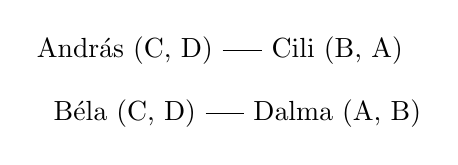
\begin{tikzpicture}
\node(A){András (C, D)};
\node(B)[below = 0.2cm of A]{Béla (C, D)};
\node(C)[right = 0.5cm of A]{Cili (B, A)};
\node(D)[below = 0.2cm of C]{Dalma (A, B)};
\draw (A) -- (C);
\draw (B) -- (D);
\end{tikzpicture}}

Erre a párosításra Béla és Cili instabilitást jelent: jobban tetszenek egymásnak, mint amennyire a párosításbeli párjuk tetszik nekik.

\textbf{Kérdés:} van-e olyan (teljes) párosítás, amelyekre nézve nincs instabilitási tényező?\\
A példában igen:

\fbox{
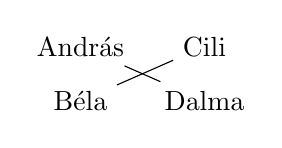
\begin{tikzpicture}
\node(A){András};
\node(B)[below = 0.2cm of A]{Béla};
\node(C)[right = 0.5cm of A]{Cili};
\node(D)[below = 0.2cm of C]{Dalma};
\draw (A) -- (D);
\draw (B) -- (C);
\end{tikzpicture}
}

\subsection*{Algoritmus tervezése}
Teljes párosítás, instabilitás nélkül $\rightarrow$ stabil házasítás.\\
\textbf{Kérdés (újra):} tetszőleges preferencialistához van-e stabil házasítás?
Ha van, akkor hogyan található ilyen (gyorsan)?

\subsubsection*{Naiv algoritmus}
\begin{itemize}
    \item Kiindulunk egy tetszőleges $M_{0}$ teljes párosításból.
    \item Ha található instabilitást jelentő f fiú és l lány erre a párosításra, akkor cseréljük a "négyesben" a párokat $\rightarrow$ $M_{1}$ párosítás.
    \item Ezt addig ismételjük, amíg található instabilitás.
\end{itemize}

\textbf{Pozitívum}: megállás után stabil házasításunk van.\\
\textbf{Negatívum}: nem feltétlenül terminál az algoritmus.

\subsubsection*{Közgazdasági Nobel-díjas algoritmus}
Gale-Shapley algoritmus (1962).
Ez egy házasítási rituálénak is felfogható, ami több napig tart.
\begin{itemize}
    \item Minden reggel a lányok kiállnak az erkélyükre és várják hogy a fiúk jöjjenek szerenádozni.
    \item Minden fiú ahhoz a lányhoz megy szerenádozni, aki a legjobban tetszik neki azok közül, akiktől még nem kapott kosarat.
    \item Ha valamelyik fiú már minden lánytól kosarat kapott, otthon marad másnap.
    \item Ha egy lány erkélye alatt legalább egy fiú szerenádozik, akkor a lány a szerenádozói közül a neki legjobban tetszőnek azt mondja, hogy várja másnap is, a többinek meg azt, hogy ne jöjjenek többet mert semmiképp nem lesz a feleségük (kikosarazás).
    \item Este azok a fiúk, akiket kikosaraztak, kihúzzák a kikosarazó lányt a preferencialistájukról.
\end{itemize}

\textbf{Megállási feltétel:} minden lány erkélye alatt LEGFELJEBB egy fiú szerenádozik.\\
\textbf{Párosítás a terminálás után:} lány $\leftrightarrow$ ablaka alatt szerenádozó fiú.


\subsection*{Algoritmus elemzése}
\subsubsection*{Hatékonyság}
\begin{itemize}
    \item legrosszabb esetben hány napig tart (egyáltalán befejeződik-e véges sok lépésben)
\end{itemize}

\textbf{Állítás:} az algoritmus legfeljebb az $(n^{2}+1)$. napon befejeződik.\\
\textbf{Bizonyítás:}
Egy olyan nap, amikor az algoritmus nem fejeződik be, van olyan lány, akinek az erkélye alatt legalább két fiú szerenádozik, következésképpen van olyan fiú, aki kosarat kap és kihúz egy lányt a preferencialistájáról.
Kezdetben a fiúk preferencialistájának összhossza $n^{2}$.
Ha a megállás előtt ezekről minden nap legalább egy lány kihúzásra kerül, akkor az $(n^{2}+1)$. napon már nincs kit kihúzni.
Következésképpen ekkorra az algoritmus biztosan befejeződik.

\subsubsection*{Helyesség}
\begin{itemize}
    \item teljes párosítás
    \item stabilitás
\end{itemize}

\textbf{Állítás:} az algoritmus teljes párosítást ad.\\
\textbf{Bizonyítás:} Indirekt tegyük fel, hogy a párosítás nem teljes.
Ekkor van olyan fiú, akinek nincs párja. Ez úgy lehetséges, hogy mindenkinél szerenádozott és mindenkitől kosarat kapott.
Ezen kívül kell lenni olyan lánynak akinek nincs párja.
Ez úgy lehetséges, hogy nála soha senki nem szerenádozott.

\textbf{Állítás:} az algoritmus stabil párosítást ad.\\
\textbf{Bizonyítás:} Indirekt tegyük fel, hogy létezik instabilitási tényező.
Azaz f-nek jobban tetszik l' mint l és l'-nek jobban tetszik f mint f'.

\fbox{\begin{tikzpicture}
\node(f){f};
\node(l)[right = 0.5cm of f]{l};
\node(f')[below = 0.5cm of f]{f'};
\node(l')[below = 0.5cm of l]{l'};
\draw (f) -- (l);
\draw (f') -- (l');
\draw[dashed] (f) -- (l');
\end{tikzpicture}}

Az f előbb szerenádozott l'-nél, mint l-nél (és l'-nél kosarat kapott).
Az l' a szerenádozói közül viszont a neki legjobban tetszőnek lesz végül a párja, ellentmondva annak, hogy l'-nek jobban tetszik f, mint f'.
\clearpage
\section {előadás (2025. szeptember 16.)}
Könyv: \url{../konyv.pdf#page=108}
\subsubsection*{Ismétlés}
\textbf{Gale-Shapley algoritmus: } tetszőleges preferencialisták esetén generál (egy) stabil párosítást.\\
\textbf{Megjegyzés: } a stabil párosítások száma akár exponenciálisan nagy lehet (n-ben).\\
\textbf{Megjegyzés: } időnként egész "egzotikus" stabil párosítások is előfordulnak, pl. az összes fiú/lány a preferencialistájának első/utolsó lányát/fiúját kapja.

\subsubsection*{Optimalitás}

Egy adott fiú és adott lány \textbf{szóba jönnek egymásnak}, ha van olyan stabil párosítás, amelyben ők egy párt alkotnak.\\
Egy adott fiú és adott lány \textbf{lelki társa} egymásnak, ha minden stabil párosításban ők egy párt alkotnak.\\

\textbf{Állítás}
\begin{itemize}
    \item \textbf{A: } az algoritmus minden fiúhoz a számára szóba jövő lányok közül a neki legjobban tetszőt párosítja.
    \item \textbf{B: } algoritmus minden lányhoz a számára szóba jövő fiúk közül a neki legkevésbé tetszőt párosítja.
\end{itemize}

\textbf{Bizonyítás}\\
\textbf{A)}

Indirekt tegyük fel, hogy van olyan fiú, akihez a Gale-Shapley algoritmus a számára szóba jövő lányok közül nem a neki legjobban tetszőt párosítja.
Ekkor ez a fiú valamelyik nap szerenádozik a számára szóba jövő lányok közül a neki legjobban tetszőnél, akitől kosarat kap.
Tekintsük azt a napot, amikor egy ilyen szomorú esemény először fordul elő.
Legyen a kosarat kapó fiú $f$ és a kosarat kapó lány $l$, és $f'$ az a fiú, aki miatt $f$ kosarat kapott.

Ekkor $l$-nek jobban tetszik $f'$, mint $f$.
Mivel az első olyan napon vagyunk, amikor egy fiút kikosaraz a számára szóba jövő lányok közül a neki legjobban tetsző, $f'$-t nem kosarazhatta még ki a számára szóba jövő lányok közül a neki legjobban tetsző $l^*$.
Egy $l^*$ nem lehet $l$ előtt $f'$ preferencialistáján ($l^*=l$ lehetséges).

Ezek után tekintsünk egy olyan $M$ stabil párosítást, amelyben $f$ és $l$ egy párt alkotnak.
Ez különbözik a Gale-Shapley algoritmus által meghatározott párosítástól.
Jelölje $l''$ az $f'$ $M$-beli párját. Mivel $l''$ szóba jön $f'$ számára, $l''$ nem lehet $l^*$ előtt $f'$ preferencialistáján ($l''=l^*$ lehetséges).

\textbf{Konklúzió: } $f' \rightarrow (l, l^*, l'')$, azaz $f'$-nek jobban tetszik $l$, mint $l''$

\textbf{Illusztráció ($M$-ben a párok):}

\fbox{\begin{tikzpicture}
\node(f){f};
\node(l)[right = 0.5cm of f]{l};
\node(f')[below = 0.5cm of f]{f'};
\node(l'')[below = 0.5cm of l]{l''};
\draw (f) -- (l);
\draw (f') -- (l'');
\draw[dashed] (f') -- (l);
\end{tikzpicture}}

Az eredeti feltevésünk szerint $f'$ és $l$ instabilitás ($M$-re) $\rightarrow$ \textbf{ellentmondás}.

\textbf{B)}

Indirekt tegyük fel, hogy van olyan lány, akihez a Gale-Shapley algoritmus a számára szóba jövő fiúk közül nem a neki legkevésbé tetszőt párosítja.
Legyen $l$ egy ilyen lány.
Legyen $M$ egy olyan stabil párosítás, amelyben $l$ párja $f$, kevésbé tetszik $l$-nek, mint a Gale-Shapley algoritmus szolgáltatta $f'$ párja.
Legyen $f'$ $M$-beli párja $l'$.

\textbf{Illusztráció ($M$-ben a párok):}

\fbox{\begin{tikzpicture}
\node(f){f};
\node(l)[right = 0.5cm of f]{l};
\node(f')[below = 0.5cm of f]{f'};
\node(l')[below = 0.5cm of l]{l'};
\draw (f) -- (l);
\draw (f') -- (l');
\end{tikzpicture}}

Most a feltételünk szerint $l$-nek jobban tetszik $f'$, mint $f$.
Másrészt a Gale-Shapley algoritmus $f'$-höz a szóba jövő lányok közül a neki legjobban tetszőt párosítja, következésképpen $f'$-nek jobban tetszik $l$ (Gale-Shapley-beli párja), mint $l'$ ($M$-beli párja).
Egy $f'$ és $l$ instabilitás ($M$-re) $\rightarrow$ \textbf{ellentmondás}.

\subsubsection*{Egyértelműség}
Futtassuk le a Gale-Shapley algoritmust úgy, hogy a fiúk szerenádoznak $\rightarrow M_1$.\\
Ezután futtassuk le úgy, hogy a lányok szerenádoznak $\rightarrow M_2$.

$M_1$ és $M_2$ stabil párosítások.\\
Ha $M_1 \neq M_2$, akkor van legalább két különböző stabil párosítás.\\
Ha $M_1 = M_2$, akkor ez az egyetlen stabil párosítás.
Mivel ez egyben fiú-optimális és fiú-pesszimális, valamint lány-optimális és lány-pesszimális, mindenki számára pontosan egy ellenkező nemű jön szóba.

\subsubsection*{Stabil szobatárs probléma (unisex változat)}
$2n$ fiú van. Mindenkinek van egy preferencialistája a többiekről.
2 ágyas szobákba szeretnénk beosztani őket.\\
Instabilitás: $\left[f_i-f_j\right]$ és $\left[f_k-f_l\right]$\\
$f_i$ szívesebben lenne $f_k$-val egy szobában, mint $f_j$-vel.\\
$f_k$ szívesebben lenne $f_i$-vel egy szobában, mint $f_l$-lel.\\
Nem feltétlenül van stabil párosítás.

\clearpage
\section {előadás (2025. szeptember 23.)}
\subsection{Stabil házasítás}
Gale-Shapley algoritmus: arra optimalizált, hogy a fiúk a lehető legjobban járjanak. Most azt szeretnénk, hogy átlagosan mindenki a lehető legjobban járjon (pl. randiapp).\\
\textbf{Állítás (pareto optimalitás):} nincs olyan teljes párosítás (nem stabil sem), amelynél minden fiú jobban jár, mint a Gale-Shapley algoritmus által szolgáltatott párosításnál.

\subsubsection*{További optimalizálási változatok}
\textbf{Jelölés:} $r_f(l) \rightarrow$ hányadik az $l$ lány az $f$ fiú preferencialistáján\\
\textbf{Jelölés:} $r_l(f) \rightarrow$ hányadik az $f$ fiú az $l$ lány preferencialistáján

\begin{enumerate}
    \item legyen $M$ stabil párosítás és tekintsük minden $l$ lányra és $f$ fiúra, ahol $(f, l) \in M$ az $r_f(l)$ és $r_l(f)$ értékeket.
    \item Keressük azt az $M$ stabil párosítást, amelyre:
    \begin{enumerate}
        \item az $r_f(l)$ és $r_l(f)$ értékek közül a legnagyobb a lehető legkisebb (mindenki a lehető legjobban jár)
        \item az $r_f(l)$ és $r_l(f)$ összege a lehető legnagyobb (mindenki a lehető legjobban jár)
        \item az $r_f(l)$ értékek összegének és az $r_l(f)$ értékek összegének különbségének abszolútértéke a lehető legkisebb (kb. egyenlően jól jár mindkét nem)
    \end{enumerate}
\end{enumerate}

\textbf{Megjegyzés:} (a)-(b): polinom időben megoldható, (c): NP-nehéz

\subsection{Algoritmustervezési módszerek}
\begin{enumerate}
    \item Oszd meg és uralkodj (pl. összefésüléses rendezés)
    \item Randomizálás (pl. gyorsrendezés)
    \item Dinamikus programozás (pl. Floyd-Warshall algoritmus)
    \item Mohó algoritmusok (pl. Kruskal, Prim, Dijkstra algoritmus)
    \item Közelítő (approximációs) algoritmusok (pl. utazó ügynök)
\end{enumerate}

\subsection{Oszd meg és uralkodj algoritmusok}
Könyv: \url{../konyv.pdf#page=8}

\textbf{Séma:}
\begin{enumerate}
    \item A feladatot hasonló, csak méretű részfeladatokra bontjuk.
    \item A részfeladatokat rekurzívan megoldjuk (ha a mérete elég kicsi, akkor közvetlenül oldjuk meg).
    \item A részfeladatok megoldását összekombináljuk az eredeti feladat megoldásává 
\end{enumerate}

\subsubsection*{Algoritmus elemzése}
\begin{itemize}
    \item helyesség
    \item hatékonyság
\end{itemize}

\textbf{Legegyszerűbb algoritmusok}
\begin{itemize}
    \item $a >= 1$ részfeladat
    \item ha $n$ az eredeti feladat mérete, akkor $n/b$ az összes részfeladat mérete, ahol $b > 1$
    \item a harmadik fázis költsége $f(n) >= 0$
    \item ha $f(n)$ jelöli az algoritmus költségét (lényeges lépések száma), akkor $T(n) = a \cdot T(n/b) + f(n)$
    \item pl. összefésüléses rendezésnél $T(n) = 2T(n/b) + n$
\end{itemize}

Összehasonlítás más algoritmusok hatékonyságával: zárt képlet.
Ilyen egyszerű rekurziókra kézzel levezethető zárt képlet.
Az egyszerűség kedvéért tfh. $n=2^k$ kettő hatvány.

"Önmagába helyettesítés":
\begin{flalign*}
T(n) &= n + \text{\fbox{$2T\left(\frac{n}{2}\right)$}} &&\\
&= n + 2\left(\frac{n}{2} + 2T\left(\frac{\frac{n}{2}}{2}\right)\right) &&\\
&= n + n + 2^2 T\left(\frac{n}{2^2}\right) &&\\
&= 2n + 2^2 \text{\fbox{$T \left(\frac{n}{2^2}\right)$}} &&\\
&= 2n + 2^2 \left(\frac{n}{2^2} + 2T\left(\frac{\frac{n}{2^2}}{2}\right)\right) &&\\
&= 2n + n + 2^3 T \left(\frac{n}{2^3}\right) &&\\
&= 3n + 2^3 T \left(\frac{n}{2^3}\right) &&\\
&\vdots &&\\
&= i n + 2^i T \left(\frac{n}{2^i}\right) &&\\
&\vdots &&\\
&= k n + 2^k T \left(\frac{n}{2^k}\right) &&\\
&= k n + 2^k T \left(\frac{n}{1}\right) &&\\
&= (1) = 0 \text{, hiszen az egyelemű tömbök rendezettek.}
\end{flalign*}

Így $T(n) = k = n$.
De $n = 2^k \rightarrow k = \log_2 n$, ezért $T(n) = n \log_2 n$.
Általánosítva (nem bizonyítjuk): mester tétel.
\subsubsection*{Mester-tétel}
Könyv: \url{../konyv.pdf#page=10}\\
Zárt formula $T(n) = a T\left(\frac{n}{b}\right) + f(n)$ formájú rekurziókhoz (nem fed le mindent).\\
$\left[f(n) \text{-t hasonlítjuk össze $n^{\log_b a}$-val} \right]$.

3 eset:
\begin{enumerate}
    \item ha $f(n) = \mathcal{O}(n^{\log_b a - \mathcal{E}})$ valamilyen pozitív $\mathcal{E}$-nal, akkor $T(n) = \Theta(n^{log_b a})$
    \item ha $f(n) = \Theta(n^{log_b a})$, akkor $T(n) = \Theta(n^{\log_b a} log n)$
    \item ha $f(n) = \Omega(n^{\log_b a + \mathcal{E}})$ valamely pozitív $\mathcal{E}$-nal ÉS $a f(\frac{n}{b}) \leq c f(n)$ valamely $c < 1$ és n elég nagy esetén, akkor $T(n) = \Theta(f(n))$
\end{enumerate}

\clearpage
\section{előadás (2025. szeptember 30.)}
\subsubsection*{Gyors mátrixszorzás}
Könyv: \url{konyv.pdf#page=12}

\textbf{Feladat:} $\underset{p \times q}{A}$ és $\underset{q \times r}{B}$ kompatibilis mátrixok AB szorzatának kiszámítása.

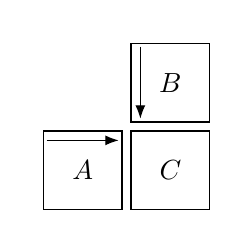
\begin{tikzpicture}[
    squarenode/.style={rectangle, draw=black, minimum width=1cm, minimum height=1cm},
]
\node[squarenode](A){$A$};
\node[squarenode](B)[above right = 0.1cm and 0.1cm of A]{$B$};
\node[squarenode](C)[right = 0.1cm of A]{$C$};
\node(A_left)[above left = -0.25cm and -0.05cm of A]{};
\node(A_right)[above right = -0.25cm and -0.05cm of A]{};
\node(B_top)[above left = -0.05cm and -0.25cm of B]{};
\node(B_bottom)[below left = -0.05cm and -0.25cm of B]{};
\draw[-Latex] (A_left) -- (A_right);
\draw[-Latex] (B_top) -- (B_bottom);
\end{tikzpicture}

$\underset{p \times r}{C} = \underset{p \times q}{A} \cdot \underset{q \times r}{B}$\\
$c_{ij} = \overset{q}{\underset{k=1}{\sum}} a_{ik} \cdot b_{kj} \rightarrow$ 1 elem kiszámításához $q$ db elemi szorzás és $q-1$ db elemi összeadás kell.\\
$p \times r$ darab elem $\rightarrow pqr$

Ha ezek mind $n \times n$-es mátrixok:
\begin{itemize}
    \item $M(n) = n^3 \in \Theta(n^3)$ (M az elemi szorzások száma)
    \item $S(n) = n^3 \in \Theta(n^3)$ (S az elemi összeadások száma)
\end{itemize}
Cél: ennél hatékonyabb algoritmus.

Ha A, B, C nem négyzetes, 0-ákkal feltöltjük:\\
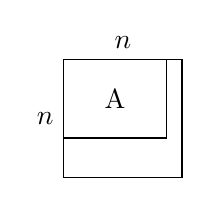
\begin{tikzpicture}[
    squarenode/.style={rectangle, draw=black, minimum size=1.5cm},
    rectanglenode/.style={rectangle, draw=black, minimum width=1.3cm, minimum height=1cm}
]
\node[squarenode](square){};
\node[rectanglenode](rect)[above left = -1.015cm and -1.315cm of square]{A};
\node[left = 0cm of square.west]{$n$};
\node[above = 0cm of square.north]{$n$};
\end{tikzpicture}
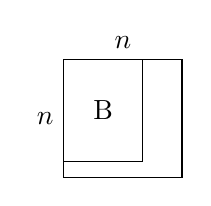
\begin{tikzpicture}[
    squarenode/.style={rectangle, draw=black, minimum size=1.5cm},
    rectanglenode/.style={rectangle, draw=black, minimum width=1cm, minimum height=1.3cm}
]
\node[squarenode](square){};
\node[rectanglenode](rect)[above left = -1.315cm and -1.015cm of square]{B};
\node[left = 0cm of square.west]{$n$};
\node[above = 0cm of square.north]{$n$};
\end{tikzpicture}

Oszd meg és uralkodj ötlet:\\
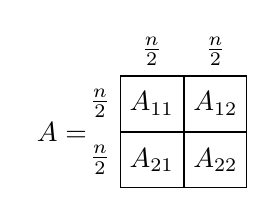
\begin{tikzpicture}[
    squarenode/.style={rectangle, draw=black, minimum size=0.7cm},
]
\node[squarenode](a11){$A_{11}$};
\node[squarenode](a12)[right = 0cm of a11]{$A_{12}$};
\node[squarenode](a21)[below = 0cm of a11]{$A_{21}$};
\node[squarenode](a22)[right = 0cm of a21]{$A_{22}$};
\node[left = 0cm of a11]{$\frac{n}{2}$};
\node[above = 0cm of a11]{$\frac{n}{2}$};
\node[above = 0cm of a12]{$\frac{n}{2}$};
\node[left = 0cm of a21]{$\frac{n}{2}$};
\node[left = 0.7cm of $(a11)!0.5!(a21)$]{$A=$};
\end{tikzpicture}
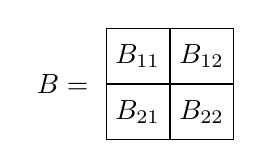
\begin{tikzpicture}[
    squarenode/.style={rectangle, draw=black, minimum size=0.7cm},
]
\node[squarenode](b11){$B_{11}$};
\node[squarenode](b12)[right = 0cm of b11]{$B_{12}$};
\node[squarenode](b21)[below = 0cm of b11]{$B_{21}$};
\node[squarenode](b22)[right = 0cm of b21]{$B_{22}$};
\node[left = 0.5cm of $(b11)!0.5!(b21)$]{$B=$};
\end{tikzpicture}
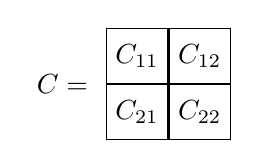
\begin{tikzpicture}[
    squarenode/.style={rectangle, draw=black, minimum size=0.7cm},
]
\node[squarenode](c11){$C_{11}$};
\node[squarenode](c12)[right = 0cm of c11]{$C_{12}$};
\node[squarenode](c21)[below = 0cm of c11]{$C_{21}$};
\node[squarenode](c22)[right = 0cm of c21]{$C_{22}$};
\node[left = 0.5cm of $(c11)!0.5!(c21)$]{$C=$};
\end{tikzpicture}

Az $A$ és $B$ mátrixok helyett 4-4 db $\frac{n}{2} \times \frac{n}{2}$-es mátrix.
\begin{flalign*}
    C_{11} &= A_{11} \cdot B_{11} + A_{12} \cdot B_{21}&&\\
    C_{12} &= A_{11} \cdot B_{12} + A_{12} \cdot B_{22}&&\\
    C_{21} &= A_{21} \cdot B_{11} + A_{22} \cdot B_{12}&&\\
    C_{22} &= A_{21} \cdot B_{12} + A_{12} \cdot B_{22}
\end{flalign*}

Elemi szorzások száma:
$
M(n) =
\begin{cases}
    1 & n=1\\
    8M\left(\frac{n}{2}\right) & n \geq 2\\
\end{cases}
$  

Elemi összeadások száma:
$
S(n) =
\begin{cases}
    0 & n=1\\
    8S\left(\frac{n}{2}\right) + 4\left(\frac{n}{2}^2\right) & n \geq 2\\
\end{cases}
$

\textbf{Kérdés: hatékonyabb-e ez a módszer?}

Csökkent-e az $M(n)$ és $S(n)$ érték?
Használjuk a Mester tételt: $T(n) = a \cdot T\left(\frac{n}{b}\right) + f(n)$

\begin{itemize}
    \item $M(n) = 8M\left(\frac{n}{2}\right)$
    \item $a = 8$, $b = 2$, $f(n) = 0$
    \item $n^{\log_2 8} = n^3$
\end{itemize}

M.T. 1. eset: ha $f(n) \in \mathcal{O}(n^{log_b a} - \mathcal{E})$ valamilyen $\mathcal{E} > 0$-ra (pl. $\mathcal{E}=0.5$), akkor $M(n) \in \Theta(n^3)$.

\begin{itemize}
    \item $S(n) = 8M\left(\frac{n}{2}\right) + n^2$
    \item $a = 8$, $b = 2$, $f(n) = n^2 \in \mathcal{O}(n^{\log_2 8 - \mathcal{E}})$, pl. $\mathcal{E}=0.5$
    \item $n^{\log_2 8} = n^3$
\end{itemize}

M.T. 1. eset $\rightarrow S(n) \in \Theta(n^3)$.

Sajnos az elemi műveletek száma nem javult, nem nyertünk semmit.

Volker Strassen észrevétele: 7 db $\frac{n}{2} \times \frac{n}{2}$-es szorzással is megkaphatjuk az eredményt.
\begin{flalign*}
    P_1 &= A_{11} \cdot (B_{12} - B_{22}) &&\\
    P_2 &= (A_{11} + A_{12}) \cdot B_{22} &&\\
    P_3 &= (A_{21} + B_{22}) \cdot B_{11} &&\\
    P_4 &= A_{22} \cdot (B_{21} - B_{11}) &&\\
    P_5 &= (A_{11} + A_{22}) \cdot (B_{11} + B_{22}) &&\\
    P_5 &= (A_{12} - A_{22}) \cdot (B_{21} + B_{22}) &&\\
    P_5 &= (A_{11} - A_{21}) \cdot (B_{11} + B_{12})
\end{flalign*}
\begin{flalign*}
    C_{11} &= P_5 + P_4 - P_2 + P_6 &&\\
    C_{12} &= P_1 + P_2 &&\\
    C_{21} &= P_3 + P_4 &&\\
    C_{22} &= P_5 + P_1 - P_3 - P_7
\end{flalign*}

Összesen:
\begin{itemize}
    \item 7 db szorzás (7 db rekurzív hívás $\frac{n}{2} \times \frac{n}{2}$ méretű mátrixokra)
    \item 18 db összeadás
\end{itemize}

$
M(n) =
\begin{cases}
    1 & n=1\\
    7M\left(\frac{n}{2}\right) & n \geq 2\\
\end{cases}
$
 és 
$
S(n) =
\begin{cases}
    0 & n=1\\
    7S\left(\frac{n}{2}\right) + 18\left(\frac{n}{2}^2\right) & n \geq 2\\
\end{cases}
$

M.T. ezekre a rekurzív függvényekre:
\begin{itemize}
    \item $M(n) = 7M\left(\frac{n}{2}\right)$
    \item $a = 7$, $b = 2$, $f(n) = 0$
\end{itemize}

M.T. 1. eset: mivel $f(n) \in \mathcal{O}(n^{log_2 7} - \mathcal{E})$ valamilyen $\mathcal{E} > 0$-ra (pl. $\mathcal{E}=0.5$), ezért $M(n) \in \Theta(n^{log_2 7})$.


\begin{itemize}
    \item $S(n) = 7S\left(\frac{n}{2}\right) + \frac{9}{2}n^2$
    \item $a = 7$, $b = 2$, $f(n) = 4.5n^2$
    \item $n^{\log_2 7} = n^{2.81}$
\end{itemize}

M.T. 1. eset: mivel $f(n) \in \mathcal{O}(n^{log_2 7} - \mathcal{E})$ pl. $\mathcal{E}=0.1$, ezért $S(n) \in \Theta(n^{log_2 7})$.
\begin{flalign*}
    C_{12}
    &= P_1 + P_2 &&\\
    &= A_{11}(B_{12} - B_{22}) + (A_{11} + A_{12}) B_{22} &&\\
    &= A_{11}B_{12} - \text{\st{$A_{11}B_{22}$}} + \text{\st{$A_{11}B_{22}$}} + A_{11}B_{22}
\end{flalign*}
$C_{21}$ hasonlóan
\begin{flalign*}
    C_{11} &= P_5 + P_4 - P_2 + P_6 &&\\
    &= (A_{11} - A_{22})(B_{11} + B_{22}) + A_{21}(B_{21}-B_{11})-(A_{11} + A_{12})B_{22} + (A_{12}-A_{22})(B_{21}+B_{22}) &&\\
    &= \cdots
\end{flalign*}

\textbf{HF.} kérdés: adott $A, B, C \in \mathcal{R}^{n \times n}$ mátrixok esetén a számolások elvégzése nélkül eldönthető-e, hogy AB = C?

\clearpage
\subsection{Randomizált algoritmusok}
\begin{itemize}
    \item Las Vegas típusú: sosem téved, de néha lassú, pl. quicksort
    \item Monte Carlo típusú: gyors, de néha téved, pl. Freivalds algoritmus
\end{itemize}

\subsubsection*{Freivalds algoritmus}
\begin{itemize}
    \item Véletlenszerűen választunk egy $\alpha \in \{0, 1\}^n$ bitvektort és kiszámoljuk ($\Theta(n^2)$ költséggel) a $\beta = (AB) \cdot \alpha = A \cdot (B \alpha)$ és $\gamma = C \cdot \alpha$ vektorokat.
    \item Ha $\beta \neq \gamma$, akkor visszatérünk HAMIS válasszal (itt biztosan nem tévedtünk).
    \item Ha $\beta = \gamma$, akkor visszatérünk IGAZ válasszal (lehet, hogy tévedtünk).
\end{itemize}

\textbf{Észrevétel:} az utóbbi eset az n dimenziós $\alpha$ bitvektorok legfeljebb felére teljesülhet.
Ha $\alpha$-t véletlenszerűen választjuk, akkor a tévedés valószínűsége $\leq \frac{1}{2}$.
Az algoritmus: végezzük el ezt 100-szor egymás után $\rightarrow$ a tévedés valószínűsége $\leq (\frac{1}{2})^{100}$.

\textbf{Észrevétel bizonyítása:}\\
Ha $AB \neq C$ és valamilyen $\alpha$-ra $AB \alpha = C \alpha$, akkor
\begin{itemize}
    \item $AB-C$ mátrix nem az azonosan 0 mátrix.
    \item tfh. az $i$. sor $j$. eleme $d > 0$.
    \item legyen $\alpha'$ az a vektor, ha $\alpha$-ban a $j$. elemet átváltjuk (bit flip).
\end{itemize}
Ekkor $(AB-C) \alpha'$ $i$. koordinátája megváltozott ($-d$-re, $+d$-re), tehát $(AB-C) \alpha' \neq 0$.
Minden $\alpha$ vektorhoz találhatunk $\alpha'$ vektort, ami kimutatja az $AB \neq C$ tényt, és különböző $\alpha$ vektorokhoz különböző $\alpha'$-t kapunk $\rightarrow$ a hamis eredményt adó vektorok száma $\geq$ helyes eredményt adó vektorok száma.






\clearpage
\section{előadás (2025. október 7.)}

\subsubsection*{Polinomok szorzása}
Könyv: \url{konyv.pdf#page=16}

$A(x) = a_0 + a_1 x + a_2 x^2 + \cdots + a_{n-1} x^{n-1}$ és $B(x) = b_0 + b_1 x + b_2 x^2 + \cdots + b_{m-1} x^{m-1}$ $(n-1)$-ed és $(m-1)$-edfokú polinomok.
Határozzuk meg a szorzatpolinomot: $C(x) = A(x) \cdot B(x)$, ahol $C(x) = c_0 + c_1 x + c_2 x^2 + \cdots + c_{n+m-2} x^{n+m-2}$.

\begin{flalign*}
    \color{red}{c_0} &\color{red}{= a_0 b_0} &&\\
    \color{orange}{c_1} &\color{orange}{= a_0 b_1 + a_1 b_0} &&\\
    \color{green}{c_2} &\color{green}{= a_0 b_2 + a_1 b_1 + a_2 b_0} &&\\
    &\vdots &&\\
    c_i &= a_0 b_i + a_1 b_{i-1} + a_2 b_{i-2} + \cdots + a_{i-1} b_1 + a_i b_0
\end{flalign*}

$
\begin{bmatrix}
    \color{red}{a_0 b_0} & \color{orange}{a_0 b_1} & \color{green}{a_0 b_2} & \color{blue}{a_0 b_3} \\
    \color{orange}{a_1 b_0} & \color{green}{a_1 b_1} & \color{blue}{a_1 b_2} & \\
    \color{green}{a_2 b_0} & \color{blue}{a_2 b_1} & & \\
    \color{blue}{a_3 b_0} & & & 
\end{bmatrix}
$

Szorzatpolinom meghatározása: $\rightarrow c_0, c_1, c_2, \cdots, c_{n+m-2}$ értékei.
Naiv módszer költsége: $\mathcal{O}(nm)$.

\textbf{Van-e ennél hatékonyabb?}
Van! Oszd meg és uralkodj algoritmust fejlesztünk (a szokásos egyszerűsítő feltételezésekkel élünk, $n=m$ kettő hatvány).
Naiv algoritmus: elemi algebra, szofisztikált algoritmus: analízis.

\subsubsection*{Interpoláció}
Egy $(n-1)$-edfokú valós (komplex) polinomot meghatároz $n$ helyettesítési értéke $\rightarrow$ interpolációs formulák (Newton, Lagrange).

\textbf{Ötlet:} határozzuk meg az $A(x)$ és $B(x)$ polinomok helyettesítési értékeit bizonyos $z_1, z_2, \cdots$ pontokban.
Ebből meglesznek $C(x)$ helyettesítési értékei a $z_1, z_2, \cdots$ pontokban.
Ezekből határozzuk meg $C(x)$ együtthatóit.

\textbf{Boszorkányos ötlet:} ha $A(x)$ és $B(x)$ $(n-1)$-edfokú polinomok, akkor $z_1, z_2, \cdots$ legyenek a $2n$-edik komplex egységgyökök.

\subsubsection*{Komplex számok}
$a + bi$ alak, ahol $i = \sqrt{-1}$.

\begin{tikzpicture}
\node(origo){};
\node[below = 1cm of origo](ImStart){};
\node[above = 2cm of origo](ImEnd){};
\node[left = 1cm of origo](ReStart){};
\node[right = 3cm of origo](ReEnd){};
\node[below left = 0cm and 0cm of ImEnd]{Im};
\node[below left = 0cm and -0.1cm of ReEnd]{Re};
\draw[->] (ImStart) -- (ImEnd);
\draw[->] (ReStart) -- (ReEnd);
\node[right = 2cm of origo](x){};
\node[above = 1cm of origo](y){};
\node[circle, fill, inner sep=1pt][above = 1.065cm of x](point){};
\node[right = 0cm of point]{$a + bi$};
\draw (x.center) -- (point);
\draw (y.center) -- (point);
\draw[decoration={brace, raise=0.05cm, mirror}, decorate] (origo) -- (x);
\draw[decoration={brace, raise=0.05cm }, decorate] (origo) -- (y);
\node[below = 0.12cm of $(origo)!0.5!(x)$]{$a$};
\node[left = 0.12cm of $(origo)!0.5!(y)$]{$b$};
\end{tikzpicture}
\begin{tikzpicture}[scale=1.5]
\draw [->](0, -0.8)--(0, 1.4);
\draw [->](-0.8, 0)--(2, 0);
\draw [-Stealth] (0, 0)--(1, 1);
\draw (0, 0) -- (0.75, 0) arc (0:45:0.75cm);
\draw (0.45, 0.18) node{$\varphi$};
\draw (0.5, 0.7) node{$r$};
\end{tikzpicture}

Trigonometrikus alak: $r(\cos \varphi + i \sin \varphi)$\\
Exponenciális alak: $r e^2 \varphi$

\textbf{Algebra alaptétele:} minden legalább elsőfokú komplex együtthatós polinomnak van komplex gyöke.

\textbf{2n. komplex egységgyökök:} $x^{2n}-1$ gyökei.

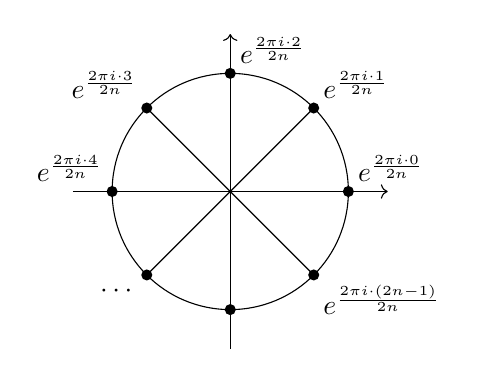
\begin{tikzpicture}
\draw [->](0, -2)--(0, 2);
\draw [->](-2, 0)--(2, 0);
\draw (0,0) circle [radius=1.5];
\fill (0, 1.5) circle(2pt) node[above right=0cm and 0cm]{$e^{\frac{2 \pi i \cdot 2}{2n}}$};
\fill (0, -1.5) circle(2pt);
\fill (1.5, 0) circle(2pt) node[above right=0cm and 0cm]{$e^{\frac{2 \pi i \cdot 0}{2n}}$};
\fill (-1.5, 0) circle(2pt) node[above left=0cm and 0cm]{$e^{\frac{2 \pi i \cdot 4}{2n}}$};
\draw (0, 0)--(1.06, 1.06);
\draw (0, 0)--(1.06, -1.06);
\draw (0, 0)--(-1.06, 1.06);
\draw (0, 0)--(-1.06, -1.06);
\fill (1.06, 1.06) circle(2pt) node[above right=0cm and 0cm]{$e^{\frac{2 \pi i \cdot 1}{2n}}$};
\fill (1.06, -1.06) circle(2pt) node[below right=0cm and 0cm]{$e^{\frac{2 \pi i \cdot (2n-1)}{2n}}$};
\fill (-1.06, 1.06) circle(2pt) node[above left=0cm and 0cm]{$e^{\frac{2 \pi i \cdot 3}{2n}}$};
\fill (-1.06, -1.06) circle(2pt) node[below left=0cm and 0cm]{$\cdots$};
\end{tikzpicture}

Jelölés: $\omega_{j, 2n} = e^{\frac{2 \pi i j}{2n}}$

\subsubsection*{Algoritmus}
\textbf{1.} $A(x)$ és $B(x)$ helyettesítési értékei a $2n.$ komplex egységgyökön oszd meg és uralkodj algoritmussal lássuk $A(x)$-nél a számítást.
Trükk: $A(x) = a_0 + a_1 x + a_2 x^2 + \cdots + a_{n-1} x^{n-1}$.

Elkészítünk két feleakkora fokszámú polinomot:
\begin{itemize}
    \item $A_{\text{páros}} = a_0 + a_2 x + a_4 x^2 + \cdots + a_{2n-2} x^{\frac{n-2}{2}}$
    \item $A_{\text{páratlan}} = a_1 + a_3 x + a_5 x^2 + \cdots + a_{n-1} x^{\frac{n-2}{2}}$
\end{itemize}

Ekkor $A(x) = A_{\text{páros}}(x^2) + A_{\text{páratlan}}(x^2)$.

\textbf{Észrevétel:} egy $2n.$ komplex egységgyök négyzete egy $n.$ komplex egységgyök: $\left(e^{\frac{2 \pi i j}{2n}}\right)^2 = e^{\frac{2 \pi i j}{n}}$.

Így $A(x)$ helyettesítési értékének kiszámítását a $2n.$ komplex egységgyökön visszavezettük két feleakkora polinom helyettesítési értékének kiszámítására az $n.$ komplex egységgyökön.
(Persze itt van még némi munka, de az $\mathcal{O}(n)$ költségű.)

\textbf{Összköltség:} $T(n) = 2T\left(\frac{n}{2}\right) + \mathcal{O}(n) \rightarrow T(n) = \mathcal{O}(n \log n)$.

\textbf{2.} $C(x) = A(x) \cdot B(x)$ helyettesítési értékeinek kiszámítása a $2n.$ komplex egységgyökön $\rightarrow \mathcal{O}(n)$.

\textbf{3.} $C(x)$ helyettesítési értékeiből a $2n.$ komplex egységgyökökön kiszámítjuk $C(x)$ együtthatóit (gyors Fourier-transzformált).

\textbf{Általánosabban:} legyen $C(x)$ legfeljebb $(2n-1)$-edfokú polinom, amelynek ismertek a helyettesítési értéki a $2n.$ komplex egységgyökökön.

Vezessük be a következő $D(x)$ polinomot:
$D(x) = d_0 + d_1 x + d_2 x^2 + \cdots + d_{2n-1} x^{2n-1}$ ahol $d_S = C(\omega_{S,2n})$ $(S = 0, 1, \cdots, 2n-1)$.

\fbox{Ekkor $D(\omega_{t, 2n}) = 2n c_{2n-t}$} (ezt még bizonyítani kell)

Alkalmazva az algoritmus oszd meg és uralkodj algoritmusát, a $D(x)$ polinomra a $D(\omega_{t, 2n})$ helyettesítési értékek, így $C(x)$ együtthatói $\mathcal{O}(n \log n)$ lépésben kiszámíthatók $\rightarrow O(n \log n)$.


\clearpage
\section{előadás (2025. október 14.)}
\subsection{Gyors Fourier transzformált}
Legyen $C(x) = c_0 + c_1 x + \cdots + c_{2n-1} x^{2n-1}$.
Tfh. ismerjük $C(x)$ helyettesítési értékeit az $\omega_{1, 2n}, \omega_{2, 2n}, \cdots, \omega_{2n, 2n}$ $2n$-edik komplex egységgyökökön.\\
Kérdés: $c_0, c_1, \cdots, c_{2n-1}$.

Bevezetünk egy $D(x) = d_0 + d_1 x + \cdots + d_{2n-1} x^{2n-1}$ polinomot, ahol $d_S = C(\omega_{S,2n})$ $(S = 0, 1, \cdots, 2n-1)$ (semmi pánik, $\omega_{0, 2n} = \omega_{2n, 2n}$).

\textbf{Állítás:} $D(\omega_{j, 2n}) = 2n c_{2n-j}$ vagyis $c_{2n-j} = \frac{1}{2n} D(\omega_{j, 2n})$ $(j = 1, 2, \cdots, 2n)$.

\textbf{Bizonyítás:}\\
\begin{flalign*}
    D(\omega_{j, 2n}) &= \overset{2n-1}{\underset{S=0}{\sum}} d_S \cdot \omega_{j, 2n}^{S} &&\\
    &= \overset{2n-1}{\underset{S=0}{\sum}} C(\omega_{S, 2n}) \cdot \omega_{j, 2n}^{S} &&\\
    &= \overset{2n-1}{\underset{S=0}{\sum}} \left( \overset{2n-1}{\underset{S=0}{\sum}} c_t \cdot \omega_{S, 2n}^{t} \right) \omega_{j, 2n}^{S}
\end{flalign*}

Kettős összegzés
\begin{figure}[H]
  \includegraphics[width=10cm]{ea/img/ea06_double_sum}
\end{figure}
"a sorrend felcserélhető"

Kitérő (C. F. Gauss):
\begin{flalign*}
    1 + 2 + \cdots + 49 + 50 = \frac{50 \cdot 51}{2} &&\\
    \underbrace{\frac{50}{51} + \frac{49}{51} + \cdots + \frac{2}{51} + \frac{1}{51}}_{50 \cdot 51}
\end{flalign*}

Visszatérve az eredeti gondolatmenethez:\\
$\overset{2n-1}{\underset{S=0}{\sum}} \left( \overset{2n-1}{\underset{t=0}{\sum}} c_t + \omega_{S, 2n}^t \right) \omega_{j, 2n}^{S} = \overset{2n-1}{\underset{t=0}{\sum}} c_t \text{\fbox{$\overset{2n-1}{\underset{S=0}{\sum}} \omega_{S, 2n}^t \cdot \omega_{j, 2n}^S$}} \text{ ez könnyen számolható:}$

\begin{flalign*}
    \omega_{S, 2n}^t \cdot \omega_{j, 2n}^S &= (e^{2 \pi i \cdot \frac{S}{2n}})^t (e^{2 \pi i \cdot \frac{j}{2n}})^S &&\\
    &= e^{2 \pi i \cdot \frac{S t}{2n}} \cdot e^{2 \pi i \cdot \frac{S j}{2n}} &&\\
    &= e^{2 \pi i \cdot \frac{S t}{2n} + 2 \pi i \cdot \frac{S j}{2n}} &&\\
    &= e^{\frac{(2 \pi i \cdot S t + 2 \pi i \cdot S j)}{2n}} &&\\
    &= e^{\frac{S \cdot 2 \pi i (t + j)}{2n}} &&\\
    &= \left(e^{\frac{2 \pi i (t + j)}{2n}}\right)^S &&\\
    &= \omega_{t+j, 2n}^S
\end{flalign*}

Az egész így:\\
$\overset{2n-1}{\underset{t=0}{\sum}} c_t \text{\fbox{$\overset{2n-1}{\underset{S=0}{\sum}} \omega_{t+j, 2n}^S$}}$

Egy pillanatra bevezetve az $\omega = \omega_{t+j, 2n}$ jelölést $\overset{2n-1}{\underset{S=0}{\sum}} \omega^S = 1 + \omega + \omega^2 + \cdots + \omega^{2n-1}$.

Vegyük észre (bizonyítsuk teljes indukcióval): $(\omega - 1)(1 + \omega + \omega^2 + \cdots + \omega^{2n-1}) = \omega^{2n} - 1$.

Mivel $\omega = \omega_{t+j, 2n}$, egy $2n$-edik komplex egységgyök, ezért $\omega^{2n} - 1 = 0$.\\
Ebből következik, hogy ha $\omega \neq 1$, akkor $1 + \omega + \omega^2 + \cdots + \omega^{2n-1} = 0$.\\
Ha $\omega = 1$, akkor $1 + \omega + \omega^2 + \cdots + \omega^{2n+1} = 1 + 1 + \cdots + 1 = 2n$.\\
Mikor lesz $\omega_{t+j, 2n} = 1$? Ha $t = 2n-j$!\\
Valóban, $t + j$ többszöröse kell, hogy legyen $2n$-nek, azonban $1 \leq j \leq 2n$ és $0 \leq t \leq 2n-1$ miatt ez csak $t+j=2n$ esetén áll fenn.

Így $\overset{2n-1}{\underset{t=0}{\sum}} c_t \underbrace{\overset{2n-1}{\underset{S=0}{\sum}} \omega_{t+j, 2n}^S}_{\text{csak $t=2n-j$ esetén $\neq 0$}} = c_{2n-j} \cdot 2n$.

\subsubsection*{Nagy egészek szorzása}
$A$, $B$ n db számjegyből áll (tízes számrendszerben felírva).\\
Kérdés: $A \cdot B = ?$

\textbf{Általános iskola}\\
\ul{234} \cdot 425\\
936\\
\- 468\\
\- 1170\\
$\overline{99450}$\\
$\mathcal{O}(n^2)$ "elemi" szorzás

\textbf{Oszd meg és uralkodj trükk} (magunk is kitalálhatjuk):

$A = A_1 \cdot 10^{\frac{n}{2}} + A_0$\\
$B = B_1 \cdot 10^{\frac{n}{2}} + B_0$\\
$A_1, A_0, B_1, B_0$ $\frac{n}{2}$ db számjegyből áll.

$AB = (A_1 \cdot 10^{\frac{n}{2}} + A_0) (B_1 \cdot 10^{\frac{n}{2}} + B_0) = A_1 B_1 \cdot 10^n + (A_1 B_0 + A_0 B_1) \cdot 10^{\frac{n}{2}} + A_0 B_0$

\textbf{Nyertünk valamit azzal}, hogy az eredeti feladatot négy feleakkora méretű feladatra redukáltuk?\\
$T(n) = 4 \cdot T(\frac{n}{2}) \rightarrow T(n) = \Theta(n^{\log_2 4}) = \Theta(n^2)$ :( \\
Azért ilyen olcsón nem várhatunk sokat!

Viszont $A_0 B_0, A_0 B_1, A_1 B_0, A_1 B_1$ helyett igazából $A_0 B_0, A_0 B_1 + A_1 B_0, A_1 B_1$ számolandó.\\
Piszkos trükk:
$(A_1 + A_0)(B_1 + B_0)$ egy szorzás.\\
Eredmény: $A_1 B_1 + \text{\fbox{$A_0 B_1 + A_1 B_0$}} + A_0 B_0$.\\
Így $A_0 B_1 + A_1 B_0 = (A_1 + A_0)(B_1 B_0) - A_1 B_1 - A_0 B_0$

Így a feladat visszavezethető csupán 3 feleakkora méretű feladatra.\\
$T(n) = 3T \left(\frac{n}{2} \right) \rightarrow T(n) = \Theta(n^{\log_2 3})$ :)

\subsection{Dinamikus programozás}
Alapelv: itt is ugyanaz, mind az oszd meg és uralkodj algoritmusoknál.
A feladatot (rekurzívan) visszavezetjük hasonló, csak kisebb méretű feladatok megoldására.

Egy tipikus oszd meg és uralkodj algoritmusnál (összefésüléses rendezés):
\begin{figure}[H]
  \includegraphics[width=10cm]{ea/img/ea06_merge_sort}
\end{figure}
Független részproblémák

Nem mindig ez a helyzet!\\
Illusztráció:\\
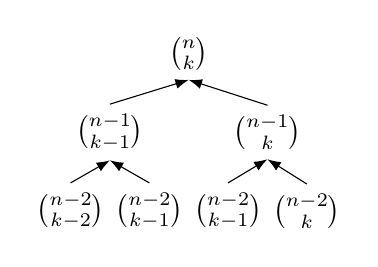
\begin{tikzpicture}
    \node(node1_1) at (0,0) {$\binom{n}{k}$};
    \node(node2_1) at (-1,-1) {$\binom{n-1}{k-1}$};
    \node(node2_2) at (1,-1) {$\binom{n-1}{k}$};
    \node(node3_1) at (-1.5,-2) {$\binom{n-2}{k-2}$};
    \node(node3_2) at (-0.5,-2) {$\binom{n-2}{k-1}$};
    \node(node3_3) at (0.5,-2) {$\binom{n-2}{k-1}$};
    \node(node3_4) at (1.5,-2) {$\binom{n-2}{k}$};
    \draw[-Latex] (node3_1.north) -- (node2_1.south);
    \draw[-Latex] (node3_2.north) -- (node2_1.south);
    \draw[-Latex] (node3_3.north) -- (node2_2.south);
    \draw[-Latex] (node3_4.north) -- (node2_2.south);
    \draw[-Latex] (node2_1.north) -- (node1_1.south);
    \draw[-Latex] (node2_2.north) -- (node1_1.south);
\end{tikzpicture}\\
"Átfedő részproblémák"

\textbf{Összefoglalva}
\begin{itemize}
    \item \textbf{Oszd meg és uralkodj} tipikusan fentről lefelé.
    \item \textbf{Dinamikus programozás} tipikusan lentről felfelé és a részproblémák megoldását egy táblázatban jegyezzük fel (létezik fentről lefelé is $\rightarrow$ memoizálás).
\end{itemize}

\textbf{Mi mindenre jó?}\\
Elhelyezünk egy sorban különböző címletű érméket, és két játékos felváltva elvehet egy érmét a sor valamelyik végéről.

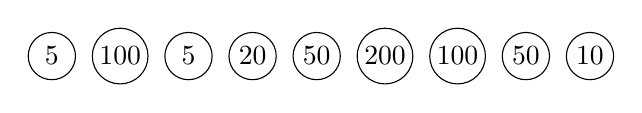
\begin{tikzpicture}[
    roundnode/.style={circle, draw=black, minimum size=0.6cm, inner sep=0.5mm}
]
\node[roundnode](c1){$5$};
\node[roundnode](c2)[right = 0.2cm of c1]{$100$};
\node[roundnode](c3)[right = 0.2cm of c2]{$5$};
\node[roundnode](c4)[right = 0.2cm of c3]{$20$};
\node[roundnode](c5)[right = 0.2cm of c4]{$50$};
\node[roundnode](c6)[right = 0.2cm of c5]{$200$};
\node[roundnode](c7)[right = 0.2cm of c6]{$100$};
\node[roundnode](c8)[right = 0.2cm of c7]{$50$};
\node[roundnode](c9)[right = 0.2cm of c8]{$10$};
\end{tikzpicture}

Milyen stratégiát kövessen Aliz az elvett érmék összértékének maximalizálására, feltéve, hogy Robi is ugyanezt akarja maga számára?
\clearpage
\section{előadás (2025. október 21.)}
\subsection{Dinamikus programozás}

Adottak az $A_1, A_2, \cdots, A_n$ mátrixok, ahol $A_1$ egy $q_0 \times q_1$ dimenziós, az $A_2$ egy $q_1 \times q_2$ dimenziós, $\cdots$, $A_n$ pedig egy $q_{n-1} \times q_n$ dimenziós mátrix.
Ekkor képezhető az $A_1 A_2 \cdots A_n$ szorzat.
A szorzatmátrix a mátrixszorzás asszociativitása miatt nem függ a zárójelezéstől.
Viszont az, hogy a szorzat kiszámítása hány elemi műveletet igényel, már általában függ a zárójelezéstől.
Az egyszerűség kedvéért tegyük fel, hogy a mátrixok szorzását a hagyományos módon végezzük: $A_{p \times q} \times A_{q \times r} = A_{p \times r}$.

Az elemi lépések most legyenek csupán az elemi szorzások.
Ekkor $p \times q \times r$ az elemi szorzások száma a szorzatmátrix kiszámításánál.

\textbf{Példa}\\
három mátrix:
\begin{flalign*}
    A_1 &\rightarrow 50 \times 5 &&\\
    A_2 &\rightarrow 5 \times 20 &&\\
    A_3 &\rightarrow 20 \times 200 &&\\
\end{flalign*}

Kétféleképpen számolhatunk:
\begin{itemize}
    \item $(A_1 A_2) A_3$
    \item $A_1 (A_2 A_3)$
\end{itemize}

Általában: határozzuk meg azt a zárójelezést, amelynek mentén a szorzat számítása a lehető legkevesebb elemi szorzással jár.

A szorzat kiszámítása nem része a feladatnak.

Az algoritmus költségét $n$ függvényében keressük, a dimenziók nem számítanak.

Első gondolat: nézzük meg az összes zárójelezést és válasszuk ki a legkedvezőbbet.

Rossz hír: a mátrixot $\Omega \left(\frac{4^n}{n^{\frac{3}{2}}}\right)$ módon lehet zárójelezni.

$\Omega \left(\frac{4^n}{n^{\frac{3}{2}}}\right) \rightarrow$ Catalan számok.

[Számos példa van.
Egy mozi pénztáránál $2n$ ember áll sorba, $n$ embernél egy ezres, a többi $n$ embernél egy kétezres van.
A mozijegy ezer forint.
A pénztárban nyitáskor üres a kassza.
Hányféleképpen állhatnak sorba az emberek, hogy mindenkinek lehessen visszaadni.]

\subsubsection*{Polinomiális algoritmus}
Tfh. az $A_1 A_2 \cdots A_n$ szorzatot akarjuk kiszámítani.
Zárójelezés $\Leftrightarrow$ szorzások sorrendje.\\
Pl. $(A_1 A_2)(A_3(A_4 A_5))$
\begin{enumerate}
    \item Első szorzás $A_1 A_2$ vagy $A_4 A_5$.
    \item Második szorzás $(A_3(A_4 A_5))$ vagy $(A_1 A_2)$. 
    \item Harmadik szorzás $A_3(A_4 A_5)$
    \item Negyedik (utolsó) szorzás $(A_1 A_2)(A_3(A_4 A_5))$
\end{enumerate}

A zárójelezés nem feltétlenül határozza meg egyértelműen a szorzások sorrendjét, de egyértelműen meghatározza az elemi szorzások számát.

\subsubsection*{Dinamikus programozás algoritmus tervezése}
\textbf{1.} Részproblémák meghatározása\\
$R[i, j] \rightarrow$ az $A_i A_{i+1} \cdots A_j$ szorzat optimális zárójelezésének meghatározása

\textbf{2.} Keressünk kapcsolatot a részproblémák optimális megoldása és a részproblémák optimális megoldása között.\\
Tegyük fel, hogy megvan $A_i A_{i+1} \cdots A_j$ optimális zárójelezése:
$\underbrace{(A_1 A_{i+1} \cdots A_k)}_{\text{ezek is zárójelezve vannak}} \underbrace{(A_{k+1} \cdots A_{j-1} A_j)}_{\text{ezek is}}$

\textbf{Állítás}\\
Az optimális zárójelezés $A_i$-től $A_k$-ig terjedő része, illetve a $A_{k+1}$-től $A_j$-ig terjedő része optimális megoldása $R[i,k]$-nak és $R[k+1, j]$-nek.

\textbf{Bizonyítás}\\
Ha lenne pl. $A_1 A_{i+1} \cdots A_k$-nak a fentinél kevesebb elemi szorzást használó kiszámítása, erre cserélve $A_{k+1} \cdots A_{j-1} A_j$ optimális zárójelezésében az $A_i \cdots A_k$ részt, egy az "optimálisnál" kevesebb elemi szorzást használó zárójelezéshez jutnánk $\rightarrow$ \textbf{ellentmondás}.

\textbf{3.} Aprópénzre váltjuk (2.)-t: rekurzió\\
Jelölje $l[i, j]$ az $R[i, j]$ optimális megoldásában az elemi szorzások számát.

Alapeset:
\begin{flalign*}
    &l[i, i] = 0 &&\\
    &l[i, i+1] = q_{i-1} q_i q_{i+1} &&
\end{flalign*}
Általában: $l[i, j] = l[i, k] + l[k+1, j] + q_{i-1} q_k q_j$

"Ne akadjunk fenn" $\rightarrow$ honnan tudjuk $k$-t?
Nem tudjuk, de $k$ biztosan $i, i+1, \cdots, j-1$ közül valamelyik.
Piszkos trükk: vizsgáljuk meg az összes lehetőséget, és válasszuk $k$-nak a legkisebb értéket adót.

$l[i, j] = \underset{i \leq j \leq j-1}{min} \{ l[i, k] + l[k+1, j] + q_{i-1} q_k q_j \}$

\textbf{4.} Számolás (3.) mentén\\
\begin{tabular}{l l l}
    $l[i, j] =$ & \raisebox{-.5\height}{\includegraphics[height=4cm]{ea/img/ea07_step4}} & $n \times n$-es táblázat \\
\end{tabular}

Költség: $\mathcal{O}(n^2)$ cella, cellánként $\mathcal{O}(n)$ számítás $\rightarrow \mathcal{O}(n^3)$

\textbf{5.} Optimális zárójelezés\\
Minden $l[i, j]$-nél megjegyezzük a minimumot adó $k$-t $\rightarrow$ backtracking a jobb felső sarokból.



\clearpage
\section{előadás (2025. november 4.)}
% Optimális zárójelezés (5. pont) folytatása

Ha az $l[i,j]$ értékek mellett feljegyezzük az optimumot adó $k$ értékeket is egy $k[i, j]$ táblázatban, akkor egy $k[1, n]$ fogja megmutatni az utolsó szorzást, pl. 9 mátrix esetén ha $k[1, 9] = 6$, akkor az optimális zárójelezés úgy néz ki, hogy
\begin{flalign*}
    &\underbrace{(A_1 A_2 \cdots A_6)}_{\text{ezek is zárójelezve vannak}} \underbrace{(A_7 A_8 A_9)}_{\text{ezek is}} &&
\end{flalign*}

Hogyan?
Általánosan:
\begin{flalign*}
    &\underbrace{(A_1 \cdots A_{k[1, n]})}_{\text{itt az első szorzás helyét ($k[1, k[1, n]]$)}} \underbrace{(A_7 A_8 A_9)}_{\text{itt pedig $k[k[1, n] + 1, n]$ helyét mutatja}} &&\\
\end{flalign*}

Az előző példát ha nézzük és azt mondjuk $k[1, 6] = 3$ és $k[1, 9] = 8$, akkor a zárójelezés egy szintet lejjebb lépve $((A_1 A_2 A_3)(A_4 A_5 A_6))((A_7 A_8) A_9)$ és így tovább.

\subsection{Sztringológia}
String-ekkel, string-ek hasonlóságával kapcsolatos kérdésekre keresünk válaszokat (gyorsan).

\subsubsection*{Az egyik legegyszerűbb ilyen kérdés}
Egy adott $T$ karaktersorozat tartalmaz-e egy adott $P$ karaktersorozatot?

Híres algoritmus: (Knuth-Morris-Pratt) $\rightarrow \Theta(|T| + |P|)$ ($|T|$ és $|P|$ a string-ek hossza)
Fő ötlet $P$ előfeldolgozása (Dinamikus Programozás).

\subsubsection*{Egy másik kérdés}
Adott egy $X$ és egy $Y$ karaktersorozat.
Keressük a leghosszabb közös részsorozatokat.
\begin{flalign*}
    & X = (x_1, x_2, \cdots, x_m) &&\\
    & Y = (y_1, y_2, \cdots, y_n) &&
\end{flalign*}

Ezeknek $Z = (z_1, z_2, \cdots, z_k)$ egy közös részsorozata lesz, ha léteznek olyan 
\begin{flalign*}
    & 1 \leq i_1 < i_2 < \cdots < i_k \leq m &&\\
    & 1 \leq j_1 < j_2 < \cdots < j_k \leq n &&
\end{flalign*}
részsorozatok, hogy
\begin{flalign*}
    & x_{i_1} = y_{j_1} = z_1 &&\\
    & x_{i_2} = y_{j_2} = z_2 &&\\
    & \cdots &&\\
    & x_{i_k} = y_{j_k} = z_k &&
\end{flalign*}

Kérdés a legnagyobb ilyen $k$.
$X$ és $Y$ hasonló, ha ez a $k$ nagy, és különböző, ha kicsi.

Például:
\begin{flalign*}
    & X = \text{\fbox{A}C\fbox{G}\fbox{C}T\fbox{A}G\fbox{C}} &&\\
    & Y =  \text{\fbox{A}T\fbox{G}\fbox{C}\fbox{A}ATC\fbox{C}} &&\\
    & Z =  \text{AGCAC} &&\\
\end{flalign*}

\subsubsection*{Egy harmadik}
Megint kiindulunk egy $X$ és egy $Y$ karaktersorozatból, de a hasonlóság definíciója kicsit más lesz.

Legyen $X = (x_1, x_2, \cdots, x_m)$ és $Y = (y_1, y_2, \cdots, y_n)$.
Az $X$ és $Y$ között bevezetjük a szekvenciaáttekintés fogalmát: ez egy párosítás az $X$-beli pozíciók és az $Y$-beli pozíciók között:
$M \subseteq \left\{ 1, 2, \cdots, m \right\} \times \left\{ 1, 2, \cdots, n \right\}$,
úgy, hogy minden $X$-beli és minden $Y$-beli legfeljebb egy $M$-beli párban fordul elő (kimaradhat pár pozíció)
ÉS ha $(i, j), (i', j') \in M$ és $i \leq i'$, akkor $j \leq j'$.

Például:

\begin{tabular}{l l l l l l l l}
    X = & A & C & G & A & C & G & T \\
        & 1 & 2 & 3 & 4 & 5 & 6 & 7
\end{tabular}

\begin{tabular}{l l l l l l l l l}
    Y = &C&A&G&A&T&G&G&A \\
        &1&2&3&4&5&6&7&8
\end{tabular}

Az $M$ szekvenciaillesztés itt lehet pl. $M = \left\{ (1, 2), (3, 3), (4, 4), (5, 6), (6, 7) \right\}$.

Vizuálisan (pozíciókat nézve):\\
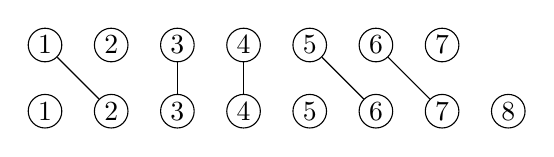
\begin{tikzpicture}[
    roundnode/.style={circle, draw=black, minimum size=0.3cm, inner sep=0.5mm}
]
\node[roundnode](t1){$1$};
\node[roundnode](t2)[right = 0.4cm of t1]{$2$};
\node[roundnode](t3)[right = 0.4cm of t2]{$3$};
\node[roundnode](t4)[right = 0.4cm of t3]{$4$};
\node[roundnode](t5)[right = 0.4cm of t4]{$5$};
\node[roundnode](t6)[right = 0.4cm of t5]{$6$};
\node[roundnode](t7)[right = 0.4cm of t6]{$7$};

\node[roundnode](l1)[below = 0.4cm of t1]{$1$};
\node[roundnode](l2)[right = 0.4cm of l1]{$2$};
\node[roundnode](l3)[right = 0.4cm of l2]{$3$};
\node[roundnode](l4)[right = 0.4cm of l3]{$4$};
\node[roundnode](l5)[right = 0.4cm of l4]{$5$};
\node[roundnode](l6)[right = 0.4cm of l5]{$6$};
\node[roundnode](l7)[right = 0.4cm of l6]{$7$};
\node[roundnode](l8)[right = 0.4cm of l7]{$8$};

\draw (t1) -- (l2);
\draw (t3) -- (l3);
\draw (t4) -- (l4);
\draw (t5) -- (l6);
\draw (t6) -- (l7);
\end{tikzpicture}


Az $i < i'$ feltétel kizárja pl. a következőt:
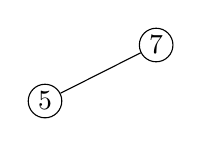
\begin{tikzpicture}[
    roundnode/.style={circle, draw=black, minimum size=0.3cm, inner sep=0.5mm}
]
\node[roundnode](l5){$5$};
\node[roundnode](t7)[above right = 0.4cm and 1.1cm of l5]{$7$};

\draw (l5) -- (t7);
\end{tikzpicture}


A szekvenciaillesztés megjeleníthető az $X$ karaktersorozatból az $Y$ karaktersorozat előállításaként karakterek törlése, beszúrása, cseréje (változatlanul hagyása) egymásutánjaként.

Az előző példában minden ferde vonalat függőlegessé teszünk:\\
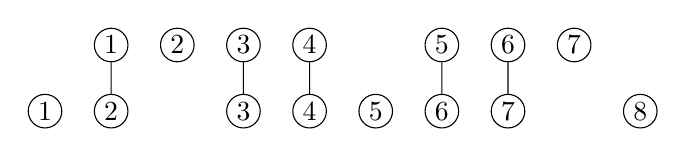
\begin{tikzpicture}[
    scale=0.84,
    roundnode/.style={circle, draw=black, minimum size=0.3cm, inner sep=0.5mm}
]
\node[roundnode](t1) at (1, 1) {$1$};
\node[roundnode](t2) at (2, 1) {$2$};
\node[roundnode](t3) at (3, 1) {$3$};
\node[roundnode](t4) at (4, 1) {$4$};
\node[roundnode](t5) at (6, 1) {$5$};
\node[roundnode](t6) at (7, 1) {$6$};
\node[roundnode](t7) at (8, 1) {$7$};

\node[roundnode](l1) at (0, 0) {$1$};
\node[roundnode](l2) at (1, 0) {$2$};
\node[roundnode](l3) at (3, 0) {$3$};
\node[roundnode](l4) at (4, 0) {$4$};
\node[roundnode](l5) at (5, 0) {$5$};
\node[roundnode](l6) at (6, 0) {$6$};
\node[roundnode](l7) at (7, 0) {$7$};
\node[roundnode](l8) at (9, 0) {$8$};

\draw (t1) -- (l2);
\draw (t3) -- (l3);
\draw (t4) -- (l4);
\draw (t5) -- (l6);
\draw (t6) -- (l7);
\end{tikzpicture}

Nézzük a betűket:

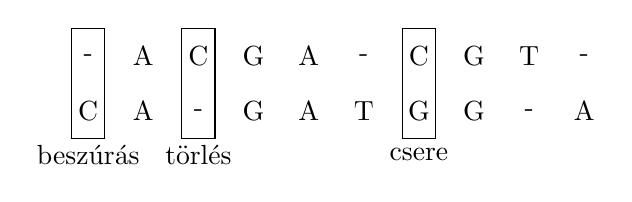
\begin{tikzpicture}[scale=0.7]
\node(t1) at (1, 1) {-};
\node(t2) at (2, 1) {A};
\node(t3) at (3, 1) {C};
\node(t4) at (4, 1) {G};
\node(t5) at (5, 1) {A};
\node(t6) at (6, 1) {-};
\node(t7) at (7, 1) {C};
\node(t8) at (8, 1) {G};
\node(t9) at (9, 1) {T};
\node(t10) at (10, 1) {-};

\node(l1) at (1, 0) {C};
\node(l2) at (2, 0) {A};
\node(l3) at (3, 0) {-};
\node(l4) at (4, 0) {G};
\node(l5) at (5, 0) {A};
\node(l6) at (6, 0) {T};
\node(l7) at (7, 0) {G};
\node(l8) at (8, 0) {G};
\node(l9) at (9, 0) {-};
\node(l10) at (10, 0) {A};

\draw (0.7,-0.5) rectangle ++(0.6,2);
\node at (1,-0.8) {beszúrás};
\draw (2.7,-0.5) rectangle ++(0.6,2);
\node at (3,-0.8) {törlés};
\draw (6.7,-0.5) rectangle ++(0.6,2);
\node at (7,-0.8) {csere};
\end{tikzpicture}

Az $X$ transzformációja $Y$-ná ennek megfelelően:
\begin{enumerate}
    \item Szúrjunk be egy C-t
    \item Másoljuk A-t
    \item Töröljük C-t
    \item Másoljuk G-t
    \item Másoljuk A-t
    \item Szúrjunk be egy T-t
    \item Cseréljük C-t G-re
    \item $\cdots$
\end{enumerate}

Persze nem csak ez az egy lehetőség van.
Melyiket használjuk a hasonlóság mérésére?

Egy $M$ szekvenciaillesztés minőségét a következőképpen definiáljuk:
\begin{enumerate}
    \item az $M$-ben nem szereplő pozíciókra felszámolunk egy fix $y > 0$ értéket (ez része az inputnak)
    \item ha $(i, j) \in M$, akkor erre felszámolunk egy $c["p", "q"] \geq 0$ értéket, ahol $x_i = "p"$ és $y_j = "q"$ (ez is része az inputnak)
\end{enumerate}

Ezeket összeadjuk, és keressük a legjobb minőségű szekvenciaillesztést, vagyis egy olyat, ahol ez az összeg minimális.

Az összes szekvenciaillesztés végigbogarászása exponenciálisan hosszú idő: $DP \rightarrow \Theta(mn)$.
Erős érvek szólnak amellett, hogy ennél polinomiálisan hatékonyabb algoritmus nem létezik.

[megjegyzés: $\theta(\frac{mn}{\log m+n})$ aszimptotikusan hatékonyabb, de polinomiálisan nem]

\subsubsection*{DP algoritmus}
Miféle részproblémák jöhetnek elő itt?
Az eddigi szerény tapasztalataink alapján: 
optimális szekvenciaillesztés $(x_i, x_{i+1}, \cdots, x_j)$, $(y_k, y_{k+1}, \cdots, y_l)$ között (infixek).

Kiderül, hogy prefixek is elegek lesznek.
$R[i, j]$ részprobléma: $(X_i) = (x_1, x_2, \cdots, x_i)$ és $(Y_j) = (y_1, y_2, \cdots, y_j)$ optimális szekvenciaillesztés meghatározása.














\clearpage
\section{előadás (2025. november 11.)}
\subsection{Optimális szekvenciaillesztés}
(Levenshtein távolság)

Pozíciók:
\begin{flalign*}
    &X = (x_1, x_2, \cdots, x_m) \rightsquigarrow \{1, 2, \cdots, m\} &&\\
    &Y = (y_1, y_2, \cdots, y_n) \rightsquigarrow \{1, 2, \cdots, n\} &&
\end{flalign*}

Egy olyan $M$ párosítást (pontosabban szekvenciaillesztést) keresünk $\{1, 2, \cdots, m\}$ és $\{1, 2, \cdots, n\}$ között, melyre a következő mennyiség minimális:
\begin{itemize}
    \item egyrészt annyiszor egy $g>0$ valós számot, ahány pozíció nem szerepel $M$-ben
    \item másrészt ha $(i, j) \subseteq M$, akkor egy $c[x_i, y_j] \geq 0$ valós számot
\end{itemize}

\subsubsection*{DP algoritmus}
\textbf{1. Részproblémák}\\
$R[i, j] \rightarrow$ optimális szekvenciaillesztés meghatározása az $X_i = (x_1, x_2, \cdots, x_i)$ és $Y_j = (y_1, y_2, \cdots, y_j)$ prefixek között.

\textbf{2. Optimális részstruktúra tulajdonság}\\
\textbf{Észrevétel}\\
Legyen $M$ szekvenciaillesztés (akármilyen) $X_i$ és $Y_j$ között.
\setulcolor{black}
Ekkor három eset lehet \ul{csak}:
\begin{enumerate}
    \item $(i, j) \in M$
    \item $i$ nem szerepel $M$-ben első tagként
    \item $j$ nem szerepel $M$-ben második tagként
\end{enumerate}

Ami hiányzik: $j$ szerepel második tagként, $i$ nem szerepel első tagként.
$(i, j) \notin M$.\\
Ám ekkor\\
\begin{tikzpicture}
\node(t1){$1$};
\node(t2)[right = 0.4cm of t1]{$2$};
\node(t3)[right = 0.4cm of t2]{$3$};
\node(b1)[below = 0.4cm of t1]{$1$};
\node(b2)[right = 0.4cm of b1]{$2$};
\node(b3)[right = 0.4cm of b2]{$3$};

\node(cdots)[right = 0.5cm of b3]{$\cdots$};
\node(ti)[right = 1cm of t3]{$i$};
\node(bj)[right = 0.5cm of cdots]{$j$};

\draw (t3) -- (bj);
\draw (b3) -- (ti);

\node[above right = 0cm and 0.7cm of bj]{$M$};
\end{tikzpicture}\\
ami nem szekvenciaillesztés.

\textbf{Állítás}\\
Legyen $M$ \ul{optimális} szekvenciaillesztés $X_i$ és $Y_j$ között.\\
Ekkor
\begin{enumerate}
    \item Ha $(i, j) \in M$, akkor $M\setminus\{(i, j)\}$ optimális szekvenciaillesztés $X_{i-1}$ és $Y_{j-1}$ között.
    \item Ha $i$ nem szerepel $M$-ben első tagként, akkor $M$ optimális szekvenciaillesztés $X_{i-1}$ és $Y_j$ között.
    \item Ha $j$ nem szerepel $M$-ben második tagként, akkor $M$ optimális szekvenciaillesztés $X_i$ és $Y_{j-1}$ között.
\end{enumerate}

\textbf{Bizonyítás}\\
\begin{enumerate}
    \item Ha $X_{i-1}$ és $Y_{j-1}$ között lenne egy $M \setminus \{(i, j)\}$-nél kedvezőbb $M^*$ szekvenciaillesztés, akkor $M^* \cup \{(i, j)\}$ egy $M$-nél kedvezőbb szekvenciaillesztés lenne $X_i$ és $Y_j$ között, \textbf{ellentmondás}.
    \item Ha lenne $X_{i-1}$ és $Y_{j}$ között egy egy $M$-nél kedvezőbb $M^*$ szekvenciaillesztés, akkor itt lenne $X_i$ és $Y_j$ között is.
    \item Analóg (2.)-hoz.
\end{enumerate}

\textbf{3. Rekurzió}\\
Jelölje $l[i,j]$ az $R[i,j]$ megoldásának "értékét".

\textbf{"Alapeset"}\\
Az egyik (vagy mindkettő) karaktersorozat üres
\begin{flalign*}
    &l[i,0] = i - g &&\\
    &l[0,j] = j + g &&
\end{flalign*}
($M = \emptyset$ az egyetlen párosítás)

\textbf{"Általában"}\\
\begin{flalign*}
    &(A) \rightarrow l[i,j] = l[i-1, j-1] + c[x_i, y_j] &&\\
    &(B) \rightarrow l[i,j] = l[i-1, j] + g &&\\
    &(C) \rightarrow l[i,j] = l[i, j-1] + g &&
\end{flalign*}

Sajnos nem tudjuk, hogy $(A)$ és $(B)$ és $(C)$ közül melyik teljesül, így mindhármat megvizsgáljuk és a legkedvezőbbet választjuk.

$
l[i, j] = min
\begin{cases}
    l[i-1, j-1] + c[x_i, y_j]\\
    l[i-1, j] + g\\
    l[i, j-1] + g
\end{cases}
$

[szakirodalomban sok helyen (bizonyítás nélkül) az áll, hogy ha $x_i = y_j$, akkor $l[i, j] = l[i-1, j-1]$ (feltéve, hogy $c["p", "q"] \geq 0$ mindig)]


\textbf{4. Optimális megoldás értéke}\\
Az $(m+1) \times (n+1)$-es $l[i,j]$ táblázatot töltjük ki fentről lefelé, soronként balról jobbra.

\begin{tabular}{l l}
    $l[i, j] =$ & \raisebox{-.5\height}{\includegraphics[width=6cm]{ea/img/ea09_matrix}} \\
\end{tabular}

Az első sorral kezdünk, az aktuális érték a három szomszédból számítódik (amiket már ismerünk) 

Számítási bonyolultság: $\mathcal{O}(mn)$ cella, cellánként $\mathcal{O}(1)$ számítás $\rightarrow \mathcal{O}(mn)$.

\textbf{5. Optimális megoldás}\\
$\rightarrow$ optimális $M$

$l[i,j]$ számításakor az $(A)$, $(B)$ és $(C)$ közül a legkedvezőbbet adót magát is feljegyezzük.

\angledarrow{0}
\angledarrow{-45}
\angledarrow{-90}
(vizuálisan)

Ezeket tároljuk egy $k[i,j]$ táblázatban, amelynek elkészülte után a jobb alsó sarokból a nyilak mentén a "margóig" lépkedünk.

Ha $k[i,j] = $ \angledarrow{135}, akkor $M = M \cup \{(i, j)\}$ az üres $M$-ből indulva.


\subsection{Leghosszabb közös részsorozat}
\begin{flalign*}
    &X = (x_1, x_2, \cdots, x_m) &&\\
    &Y = (y_1, y_2, \cdots, y_n) &&
\end{flalign*}
Egy leghosszabb olyan $Z = (z_1, z_2, \cdots, z_k)$-t keresünk, amely megkapható $X$-ből is és $Y$-ból is "néhány" karakter törlésével.

Hasonló DP algoritmus működik itt is, mint az előbb.

\fbox{\textbf{1.}} $R[i,j]$ $X_i$ és $Y_j$ egy leghosszabb közös részsorozatának meghatározása\\
\fbox{\textbf{2.}} \textbf{Állítás}\\
Legyen $Z_k = (z_1, z_2, \cdots, z_k)$ az $X_m = (x_1, x_2, \cdots, x_m)$ és $Y_n = (y_1, y_2, \cdots, y_n)$ egy leghosszabb közös részsorozata (LKR).

\begin{enumerate}
    \item Ha $x_m = y_n$, akkor $z_k = x_m = y_n$ ÉS $Z_{k-1}$ egy LKR $X_{m-1}$-hez és $Y_{n-1}$-hez.
    \item Ha $x_m \neq z_k$, akkor $Z_{k}$ egy LKR $X_{m-1}$-hez és $Y_n$-hez.
    \item Ha $y_n \neq z_k$, akkor $Z_{k}$ egy LKR $X_m$-hez és $Y_{n-1}$-hez.
\end{enumerate}

\fbox{\textbf{3.}}
Legyen $l[i, j]$ az $R[i,j]$ optimális megoldásának értéke (hossza).
\begin{flalign*}
    &(A) \rightarrow l[i,j] = l[i-1, j-1] + 1 &&\\
    &(B) \rightarrow l[i,j] = l[i-1, j] &&\\
    &(C) \rightarrow l[i,j] = l[i, j-1] &&
\end{flalign*}

$
l[i, j] = min
\begin{cases}
    0 & \text{ha $i=0$ vagy $j=0$ (rekurzió "elvarrása")}\\
    l[i-1, j-1] + 1 & \text{ha $i,j \geq 1$ és $x_i = y_j$ $(A)$}\\
    min \{l[i-1, j], l[i, j-1]\} & \text{ha $i,j \geq 1$ és $x_i \neq y_j$ $(B)$, $(C)$}\\
\end{cases}
$
\clearpage
\section{előadás (2025. november 18.)}
\subsection{NP-nehéz  feladatok és DP}

\subsubsection*{1. Részhalmaz-összeg}
(NP-teljes eldöntési feladat)

Adott $a_1, a_2, \cdots, a_n, B$ pozitív egészekhez létezik-e olyan $I \in \left\{ 1, 2, \cdots, n \right\}$, hogy $\underset{i \in I}{\sum} a_i = B$?

\subsubsection*{2. Pénzváltás}
Adott $a_1, a_2, \cdots, a_n, B$ pozitív egészekhez léteznek-e olyan $\alpha_1, \alpha_2, \cdots, \alpha_n$ nemnegatív egészek, hogy $\overset{n}{\underset{i = 1}{\sum}} \alpha_i a_i = B$?

\textbf{Optimalizálási feladat}\\
Ha a válasz igen, mi $\overset{n}{\underset{i = 1}{\sum}} \alpha_i$ minimális értéke?

\textbf{"Boltban"}\\
$B \rightarrow$ visszajáró pénz\\
$a_1, a_2, \cdots, a_n \rightarrow$ rendelkezésre álló címletek (pl. érmék)

A legkevesebb érmével akarjuk a $B$ összeget kifizetni.

Az egyszerűség kedvéért tegyük fel, hogy a címletek között szerepel az 1, mondjuk $1 = c_1 < c_2 < c_3 < \cdots < c_n$.

\textbf{Bolti algoritmus:} vegyük a legnagyobb olyan $c_i$-t, amelyre $c_i \leq B$, és adjunk belőle annyit, amennyit lehetséges.
Ezután rekurzívan fizetjük ki a maradékot.

Optimális megoldást ad az algoritmus?

A tipikus (ahol a címletek: $1c, 2c, 5c, 10c, 20c, 50c$) boltokban igen.\\
Sajnos nem minden címlethalmaznál "működik" ez: $1, 6, 10$.
\begin{flalign*}
    & 12 \rightarrow 10 + 1 + 1 \text{ algoritmus} &&\\
    & 12 \rightarrow 6 + 6 \text{ optimális} &&
\end{flalign*}
Tetszőleges $c_1, c_2, \cdots, c_n$ címletekre ez egy NP-nehéz feladat.

Meglepetés: polinom időben eldönthető, hogy adott $c_1, c_2, \cdots, c_n$ címletekre a bolti algoritmus optimális megoldást ad-e.

\subsubsection*{3. Hátizsák feladat}
Adottak az $a_1, a_2, \cdots, a_n, c_1, c_2, \cdots, c_n, B$ pozitív egész számok, határozzunk meg egy olyan $I \subseteq \left\{ 1, 2, \cdots, n \right\}$ indexhalmazt, amelyre $\underset{i \in I}{\sum} a_i \leq B$ és $\underset{i \in I}{\sum} c_i$ maximális.

Mitől hátizsák feladat ez?
Van $n$ tárgyunk $t_1, t_2, \cdots, t_n$.
A $t_i$ tárgy súlya $b_i$, értéke $c_i$.
Van egy hátizsákunk, amelynek (súly)kapacitása $B$.\\
Mely tárgyakat tegyük a hátizsákba, hogy az összérték maximális legyen, a súlykorlátot nem túllépve?

\subsubsection*{Összefüggések 1-2-3 között}
\textbf{Részhalmaz-összeg és hátizsák feladat}\\
Hogyan lehetne alkalmazni egy hátizsák feladatra adott algoritmust a részhalmaz-összeg feladat megoldására?
(visszavezetés, rekurzió)

Tekintsük a részhalmaz-összeg feladat egy példányát: $a_1, a_2, \cdots, a_n, B$

Elkészítünk ehhez egy hátizsák feladat példányt:\\
n tárgy, az $i$-edik súlya és értéke is $a_i$ \\
a hátizsák kapacitása $B$

Tegyük fel, hogy ennek a hátizsák feladatnak $I$ egy megoldása: $\underset{i \in I}{\sum} a_i \leq B$ és $\underset{i \in I}{\sum} c_i$ maximális

Két eset van:\\
$\rightarrow \underset{i \in I}{\sum} = B \rightarrow$ igen a részhalmaz-összegnél\\
$\rightarrow \underset{i \in I}{\sum} < B \rightarrow$ nem (igen esetén $I$ nem lenne optimális megoldás)

\textbf{Részhalmaz-összeg és pénzváltás}\\
(eldöntési változat)

\ul{Pénzváltás példány:}\\
$a_1, a_2, \cdots, a_n, B$
$a_1$-ből vegyünk $\left\lfloor \frac{B}{a_1} \right\rfloor$ példányt\\
$a_2$-ből vegyünk $\left\lfloor \frac{B}{a_2} \right\rfloor$ példányt\\
\vdots\\
$a_n$-ből vegyünk $\left\lfloor \frac{B}{a_n} \right\rfloor$ példányt

\ul{Részhalmaz-összeg példány:}\\
$\underbrace{a_1, \cdots, a_1}_{\left\lfloor \frac{B}{a_1} \right\rfloor}, \underbrace{a_2, \cdots, a_2}_{\left\lfloor \frac{B}{a_2} \right\rfloor}, \cdots, \underbrace{a_n, \cdots, a_n}_{\left\lfloor \frac{B}{a_n} \right\rfloor}, B$

Ha itt igen, akkor a pénzváltásnál is igen, ha nem, akkor ott is nem.

\textbf{Probléma:} a részhalmaz-összeg példány mérete nem csak $n$-től, de $B$-től is függ, ez utóbbitól lineárisan.

\textbf{Lineárisan:} ez elfogadhatatlan!
Ami elfogadható lenne itt: $\Omega(\log B)$.

Elérhető ez?
IGEN!

$a_1 \rightarrow \underbrace{a_1, 2 a_1, 4 a_1, 8 a_1, \cdots, 2^{\left\lfloor \log_2 B \right\rfloor} a_1}_{\text{\parbox{5.5cm}{\centering kettes számrendszerben gondolkodhatunk \\ $a_1, 2 a_1, 3 a_1, \cdots \left\lfloor \frac{B}{a_1} \right\rfloor a_1$ közül minden \\ felírható csupán ezeket használva}}}$

Ugyanez $a_2, a_3, \cdots, a_n$ esetén.


\clearpage
\section{előadás (2025. november 25.)}
\subsubsection*{Hátizsák feladat}
Legyenek $t_1, t_2, \cdots, t_n$ tárgyak.
Minden $t_i$ tárgynak van egy $w_i$ súlya és egy $v_i$ értéke.
Adott egy hátizsák $W$ kapacitással.
Válasszunk ki a tárgyak közül néhányat úgy, hogy a kiválasztott tárgyak összsúlya ne haladja meg a hátizsák $W$ kapacitását és az összértéke a lehető legnagyobb.

Ismert, hogy ez egy NP-nehéz feladat.
Ezzel együtt van egy különös tulajdonsága: bármely $\mathcal{E} > 0$ valós számhoz van olyan polinomiális algoritmus, amely által szolgáltatott megoldásban az összérték legalább $\frac{1}{1 + \mathcal{E}}$-szorosa az optimális összértéknek.
(aprópénzre váltva legalább $99\%$-a, legalább $99,9\%$-a, legalább $99,99\%$-a, és így tovább)

Hátizsák feladat input:
$w_1, v_1, w_2, v_2, \cdots, w_n, v_n, W$ mind pozitív egészek.

\textbf{DP algoritmus (általánosan nem polinomiális!)}\\
\textbf{1. Részproblémák}\\
$R[i,j] \rightarrow$ tárgyak $t_1, t_2, \cdots, t_i$, hátizsák kapacitás: $j$

\textbf{2. Optimális részstruktúra tulajdonság}\\
Legyen Opt egy optimális (maximális összértékű) megoldása $R[i,j]$-nek.

Most $t_i \notin$ Opt  (Opt most egy tárgyhalmaz) esetén Opt optimális megoldása $R[i-1,j]$-nek.
Valóban, ha lenne $R[i-1,j]$-nek Opt-nál nagyobb összértékű megoldása, az Opt-nál nagyobb összértékű megoldása lenne $R[i,j]$-nek is, \textbf{ellentmondás}.

Másrészt $t_i \in Opt$ esetén Opt$\setminus \left\{t_i\right\}$ egy maximális összértékű megoldása $R[i-1,j-w_i]$-nek.
Valóban, ha lenne $R[i-1, j-w_i]$-nek Opt$\setminus \left\{t_i\right\}$-nél nagyobb összértékű megoldása, akkor ezt kiegészítve $t_i$-vel, $R[i,j]$-nek egy Opt-nál nagyobb összértékű megoldását kapnánk, \textbf{ellentmondás}.

\textbf{3. Rekurzió}\\
Jelölje $h[i,j]$ az $R[i,j]$ optimális megoldásánál az összértéket.

Nyilván $h[i,0]$ és $h[0,j]$ nulla.

Különben, vagyik amikor $i, j \geq 1$, akkor 

\fbox{\textbf{A}} ha $w_i > j$, akkor $t_i$ nem lehet benne az optimális megoldásban, így $h[i,j]=h[i-1,j]$.

\fbox{\textbf{B}} ha viszont $w_i \leq j$, akkor $t_i$ vagy benne van az optimális megoldásban, vagy nincs, és nem is tudjuk melyik áll fenn a kettő közül.
Így szokásos módon mindkét lehetőséget megvizsgáljuk, és a kedvezőbb lesz a befutó:

$
h[i, j] = max
\begin{cases}
    v_i + h[i-1, j-w_i] & \text{(benne van)}\\
    h[i-1, j] & \text{(nincs benne)}\\
\end{cases}
$

\textbf{4. Táblázat}\\
Az $(n+1) \times (w+1)$-dimenziós $h[i,j]$ táblázatot töltjük ki (felülről lefelé)

\begin{tabular}{l l}
    $h[i, j] =$ & \raisebox{-.5\height}{\includegraphics[width=8cm]{ea/img/ea11_matrix1}} \\
\end{tabular}

Oszlopok: $j = 0, 1, \cdots, W$

\ul{Költség:}\\
egy cella: $\mathcal{O}(1)$\\
cellák száma: $\mathcal{O}(nW)$\\
összesen: $\mathcal{O}(nW)$, nem polinomiális!

A táblázatban az oszlopok száma $W+1$, ez $W$, mint input input méretében (ami $\log W$) exponenciálisan nagy.

Megjegyzés: kis súlyok esetén az algoritmus polinomiális (pontosítva: $w_1 + w_2 + \cdots + w_n \leq W$ esetén a feladat triviális, itt nem ilyenekről van szó)

\textbf{5. Optimális tárgyhalmaz}\\
$h[i,j]$ számolásakor feljegyezzük, hogy $t_i$ beválasztása vagy kihagyása volt kedvezőbb, a jobb alsó sarkoból indulva ezek segítségével rekonstruálható egy optimális megoldás.

\textbf{Lássunk ezek után egy alternatív megközelítést}\\
Hátizsák feladat kicsit másképpen
\begin{itemize}
    \item input változatlan
    \item "Célfüggvény" legalább V összértéket szeretnénk elérni az ehhez szükséges tárgyak minimális összsúlya mellett.
\end{itemize}

DP itt is működik (ezt talán mindenki érzi)

\textbf{1. Részproblémák}\\
$R[i,j]$ a $t_1, t_2, \cdots, t_i$ tárgyakból válaszhatunk és legalább $j$ összértéket akarunk elérni minimális összsúly mellett.

Jelölje $h^*[i,j]$ a minimális összsúlyt.

\fbox{\textbf{2.}}-\fbox{\textbf{3.}} nagyon hasonlít az előbbiekhez.

\textbf{4. Táblázat}\\
$h^*[i, j] =$
\raisebox{-.5\height}{
\begin{tikzpicture}
\node(img) {\includegraphics[width=6cm]{ea/img/ea11_matrix2}};
\node[above right=-0.5cm and -4.5cm of img]{$v_1 + v_2 + \cdots + v_i$};
\node[above right=-0.5cm and -1.3cm of img]{$v_1 + v_2 + \cdots + v_n$};

\node(arr1end) at (0.1, -0.5){};
\node(arr2end) at (2.2, -2.1){};

\node(wi) at (2.1, 0.2){$w_1 + w_2 + \cdots + w_i$};
\node(wn) at (3, -2.8){$w_1 + w_2 + \cdots + w_n$};

\draw[-Latex] (wi.south) -- (arr1end.center);
\draw[-Latex] (wn.north) -- (arr2end.center);
\end{tikzpicture}
}


Csak az "alsó" részt töltjük ki.

Hogyan használható ez a táblázat az "eredeti" hátizsák feladat megoldására (ahol $W$ a hátizsák kapacitása)?
Az utolsó sorban balról jobbra haladva megkeressük az utolsó $\leq W$ értéket, ennek oszlopindexe lesz az elérhető maximális összsúly.

\ul{Költség:}\\
egy cella: $\mathcal{O}(1)$\\
cellák száma: legyen $v^* = max v_i$\\
sorok száma: $\mathcal{O}(n)$\\
oszlopok száma: $\mathcal{O}(n v^*)$\\
összesen: $\mathcal{O}(n^2 v^*)$, nem polinomiális!

Azonban kis értékek esetén polinomiális!
Pl. ha $v^*=(n^3)$

\clearpage
\section{előadás (2025. december 2.)}
\subsubsection*{Közelítő hátizsák feladat}
\textbf{Tétel}\\
Minden $\mathcal{E} > 0$ valós számhoz létezik olyan polinomiális algoritmus, amely által visszaadott összérték a hátizsák problémára legalább $\frac{1}{1 + \mathcal{E}}$-szorosa az optimális megoldásnak.

\textbf{Hátizsák feladatunk}
\begin{flalign*}
    &t_1 \rightarrow (w_1, v_1) &&\\
    &t_2 \rightarrow (w_2, v_2) &&\\
    &\vdots &&\\
    &t_n \rightarrow (w_n, v_n) &&\\
    &W                          &&
\end{flalign*}
Nyilván azok a tárgyak, amelyek súlya nagyobb, mint W nem lehetnek benne egyetlen megoldásban sem, ezért feltehetjük, hogy $w_i \leq W (1 \leq i \leq n)$

Nyilván elég a tételt olyan $\mathcal{E}$ pozitív számokra igazolni, amelyek pozitív egészek reciprokai.

Definiálhatunk két másik hátizsák feladatot.
Legyen $b = \frac{\mathcal{E}}{2n} v^*$ (ahol $v^* = \underset{i}{max} v_i$)

A súlyok és a hátizsák kapacitása változatlan.

\fbox{\textbf{I.}} az értékek $\tilde{v}_i = \left\lceil \frac{v_i}{b} \right\rceil b$\\
\fbox{\textbf{II.}} az értékek $\hat{v}_i = \left\lceil \frac{v_i}{b} \right\rceil = \frac{\tilde{v}_i}{b}$

Jegyezzük meg, hogy $v_i \leq \tilde{v}_i \leq v_i + b$.

Nyilván \fbox{\textbf{I.}} és \fbox{\textbf{II.}} optimális megoldása ugyanaz $\rightarrow \mathcal{J}$

Oldjuk meg \fbox{\textbf{II.}}-t a múlt végén ismertetett DP algoritmussal.

\textbf{Mi is volt ez a DP algoritmus?}

A részproblémák úgy néztek ki, hogy a $t_1, t_2, \cdots, t_i$ tárgyakkal akartunk legalább $j$ értéket elérni minimális összsúly mellett $\rightarrow h^*(i,j)$ volt a min összsúly.

[$1 \leq i \leq n$, $0 \leq j \leq v_1 + v_2 + \cdots + v_i$]

Ekkor:
\begin{flalign*}
&h^*[i,j] =
\begin{cases}
    0 & \text{ha $j = 0$}\\
    w_i + h^*[i-1, max \left\{ 0, j - v_i \right\}] & \text{ha $j > v_1  + v_2 + \cdots + v_{i-1}$}\\
    min
    \begin{cases}
        w_i + h^*[i-1, max \left\{ 0, j - v_i \right\}] & \\
        h^*[i-1, j] &
    \end{cases} & \text{ha $1 \leq j \leq v_1  + v_2 + \cdots + v_{i-1}$}
\end{cases}
&&\\
\end{flalign*}

\textbf{Táblázat}\\
\begin{tikzpicture}
\node(img) {\includegraphics[width=6cm]{ea/img/ea12_matrix.pdf}};
\node[above right=-0.3cm and -3.5cm of img]{opt. mo, ez az oszlopindex};
\node[below right=-0.2cm and -4.9cm of img]{$\rightarrow$ utolsó $\leq W$ érték};

\draw[-Latex] (0.52, -2.43) -- (0.52, 2.7);
\end{tikzpicture}

Költség: n sor, $\leq n v^*$ oszlop, cellánként $\mathcal{O}(1)$ számolás $\rightarrow \mathcal{O}(n^2 v^*)$

\fbox{\textbf{II.}} megoldásának költsége\\
$\mathcal{O}(n^2 \underset{i}{max} \hat{v}_i)$

Mennyi ez?
Legyen $\underset{i}{max} v_i = v_j$.
Ekkor $\underset{i}{max} \hat{v}_i = \hat{v}_j$.

Igen ám, de
$\hat{v}_j =
\left\lceil \frac{v_j}{b} \right\rceil =
\left\lceil \frac{v^*}{b} \right\rceil =
\left\lceil \frac{v^*}{\frac{\mathcal{E}}{2n} v^*} \right\rceil = 
\left\lceil \frac{1}{\frac{\mathcal{E}}{2n}} \right\rceil = 
\left\lceil \frac{2n}{\mathcal{E}} \right\rceil = 
\frac{2n}{\mathcal{E}}
$
($\frac{1}{\mathcal{E}}$ pozitív egész, $2n$ is)

Visszahelyettesítve $\mathcal{O}(n^2 \underset{i}{max} \hat{v}_i)$-ba ez $\mathcal{O}(n^3 \mathcal{E}^{-1})$ ami rögzített $\mathcal{E}$ mellett polinomiális!

Hátra van még az "$\frac{1}{1 + \mathcal{E}}$ rész".

Idézzük fel, hogy $\mathcal{J}$ nem csak a $\hat{v}_i$ értékekkel, de a $\tilde{v}_i$ értékekkel is optimális megoldás.

Mit mondhatunk $\mathcal{J}$-ről a $v_i$ értékek esetén (eredeti hátizsák feladat)?

Tekintsük az eredeti feladat egy tetszőleges $\mathcal{J}^*$ megengedett megoldását (ebben benne van az optimális is).

Megmutatjuk, hogy $\frac{1}{1 + \mathcal{E}} \underset{i \in \mathcal{J}^*}{\sum} v_i \leq \underset{i \in \mathcal{J}}{\sum} v_i$.
Vagy kicsit átrendezve: $\underset{i \in \mathcal{J}^*}{\sum} v_i \leq (1 + \mathcal{E}) \underset{i \in \mathcal{J}}{\sum} v_i$.
(Persze $\mathcal{J}$ is egy megengedett megoldása az eredeti feladatnak, mert a súlyok és a kapacitás nem változik.)

Az optimális megoldást adó $\mathcal{J}^*$-gal ez pont a tétel állítása.

\textbf{"Bűvészkedünk"}\\
Idézzük fel, hogy $v_i \leq \tilde{v}_i \leq v_i + b$.
Most jön egy hosszú egyenlőtlenséglánc:\\
$\underset{i \in \mathcal{J}^*}{\sum} v_i \leq 
\underset{i \in \mathcal{J}^*}{\sum} \tilde{v}_i \leq 
\underset{i \in \mathcal{J}}{\sum} \tilde{v}_i \leq 
\underset{i \in \mathcal{J}}{\sum} (v_i + b) \leq 
\underset{i \in \mathcal{J}}{\sum} v_i + \underset{i \in \mathcal{J}}{\sum} b \leq 
\left(\underset{i \in \mathcal{J}}{\sum} v_i\right) + nb
$

$\mathcal{J}$ az optimális megoldás a $\tilde{v}_i$ értékekre.
Arra hajtunk, hogy $nb \leq \mathcal{E} \underset{i \in \mathcal{J}}{\sum} v_i$.

Piszkos trükk: nézzük az egyenlőtlenséglánc következő részét:
$
\underset{i \in \mathcal{J}}{\sum} \tilde{v}_i \leq 
\left(\underset{i \in \mathcal{J}}{\sum} v_i\right) + nb
$

Először is a $j$-edik tárgy (ennek a legnagyobb az értéke) önmaga megengedett megoldása \fbox{\textbf{I.}}-nél, így $\tilde{v}_j \leq \underset{i \in \mathcal{J}}{\sum} \tilde{v}_i$.

\clearpage
\section{előadás (2025. december 2.)}
\subsubsection*{Ütemezés}

Adott munkák $M = \{m_1, m_2, \cdots, m_n\}$ halmaza, és minden $m_i \in M$-hez:

\begin{itemize}
    \item $t_i$: ennyi ideig tart elvégezni
    \item $d_i$: határidő
    \item $w_i$: munkadíj
\end{itemize}

($\geq 0$ egészek)

Mely munkákat vállaljuk el a max. összdíjért?

\begin{itemize}[label=$\rightarrow$]
    \item egyszerre csak egy munkát lehet végezni
    \item nem lehet félbeszakítani
    \item határidőre be kell fejezni
\end{itemize}

Az $m_{i_1}, m_{i_2}, \cdots, m_{i_k}$ kiválasztott munkák egy megengedett ütemezése: megadunk $S_{i_1}, f_{i_1}$ értékeket, amire:
\begin{flalign*}
    &0 \leq S_{i_1}, f_{i_1} = S_{i_1} + t_{i_1}, f_{i_1} \leq d_{i_1} &&\\
    &f_{i_1} \leq S_{i_2}, f_{i_2} = S_{i_2} + t_{i_2}, f_{i_2} \leq d_{i_2} &&\\
    &f_{i_2} \leq S_{i_3}, f_{i_3} = S_{i_3} + t_{i_3}, f_{i_3} \leq d_{i_3} &&\\
    &\vdots &&\\
    &f_{i_{k-1}} \leq S_{i_{k}}, f_{i_{k}} = S_{i_{k}} + t_{i_{k}}, f_{i_{k}} \leq d_{i_{k}} &&
\end{flalign*}

Szeretnénk az $M$ olyan részhalmazát választani, aminek van megengedett ütemezése és $\overset{k}{\underset{l=1}{\sum}} w_{i_k}$ maximális.

Ez NP-nehéz feladat.
Létezik DP algoritmus a feladat megoldására.

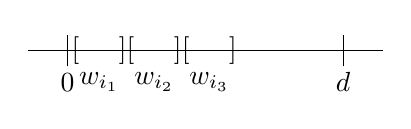
\begin{tikzpicture}
\draw (0, 0) -- (4.5, 0);
\draw (0.5, -0.2) -- (0.5, 0.2);
\draw (4, -0.2) -- (4, 0.2);

\node at (0.5, -0.4){$0$};
\node at (4, -0.4){$d$};

\node at (0.6, 0) {[};
\node at (1.2, 0) {]};
\node at (0.9, -0.4) {$w_{i_1}$};

\node at (1.3, 0) {[};
\node at (1.9, 0) {]};
\node at (1.6, -0.4) {$w_{i_2}$};

\node at (2.0, 0) {[};
\node at (2.6, 0) {]};
\node at (2.3, -0.4) {$w_{i_3}$};

\end{tikzpicture}

Speciális eset: $d_1 = d_2 = \cdots = d_n = d$.
Minden határidő ugyanaz $\rightarrow$ hátizsák probléma $t_i$ súlyokkal, $w_i$ értékkel, $d$ kapacitással.

Egy másik speciális eset: $w_1 = w_2 = \cdots = w_n$.
Cél: legtöbb munka elvégzése.
Erre van $\mathcal{O}(n \log n)$-es MOHÓ ALGORITMUS.

Mohó algoritmus az ütemezési probléma speciális esetére:\\
Feltehetjük, hogy $d_1 \leq d_2 \leq \cdots \leq d_n$.
Egy $H$ halmazba fogjuk gyűjteni a kiválasztott munkákat.
Kezdetben legyen $H = \oslash$.
Egymás után vesszük hozzá $H$-hoz az $m_1$ munkákat. $i = 1,2,3, \cdots$.

Ha az $m_i$ munka bevételével $\underset{m_j \in H}{\sum} t_j > d_i$ adódik, akkor töröljük $H$-ból a leghosszabb elvégzési idejűt.

Végül a $H$-beli feladatokat ütemezzük a 0. időpillanattól szünet nélkül a határidők szerint növekvő sorrendben (kanonikus ütemezés).

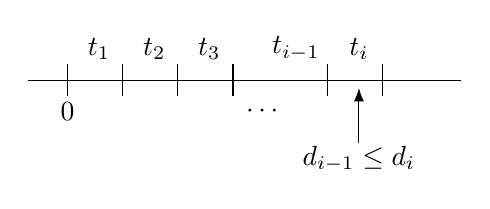
\begin{tikzpicture}
\draw (0, 0) -- (5.5, 0);

\draw (0.5, -0.2) -- (0.5, 0.2);
\draw (1.2, -0.2) -- (1.2, 0.2);
\draw (1.9, -0.2) -- (1.9, 0.2);
\draw (2.6, -0.2) -- (2.6, 0.2);

\draw (3.8, -0.2) -- (3.8, 0.2);
\draw (4.5, -0.2) -- (4.5, 0.2);

\node at (0.5, -0.4){$0$};
\node at (0.9, 0.4){$t_1$};
\node at (1.6, 0.4){$t_2$};
\node at (2.3, 0.4){$t_3$};
\node at (3.0, -0.4){$\cdots$};
\node at (3.4, 0.4){$t_{i-1}$};
\node at (4.2, 0.4){$t_i$};

\draw[-Latex] (4.2, -0.8) -- (4.2, -0.1);
\node at (4.2, -1) {$d_{i-1} \leq d_i$};
\end{tikzpicture}

\textbf{Állítás:} $H$-ban minden munka befejeződik legkésőbb a határidőre.\\
\textbf{Bizonyítás:} triviális.

\clearpage
\textbf{Állítás:} $H$ optimális ütemezés az adott munkákra nézve.\\
\textbf{Bizonyítás:}\\
Indukció $n$-re ($|M| = n$)

$n = 1$: triviális

Most tegyük fel, hogy $n > 1$ és a mohó algoritmus optimális ütemezést ad $\leq n-1$ munka esetén.

Ha $H$ tartalmazza az összes munkát, akkor optimális $\rightarrow$ kész vagyunk.

Tegyük fel, hogy $H$ nem az összes munkát tartalmazza, és legyen $m_k$ az a munka, amit először törölt a mohó algoritmus, mondjuk az $m_i$ munka hozzávételekor.

\textbf{Állítás:} van olyan $\mathcal{O}$ optimális kanonikus ütemezés, hogy $m_k$ ebben sem szerepel.\\
\textbf{Bizonyítás:} hamarosan

Hogyan használhatjuk ezt $H$ optimalitásának bizonyítására?

Nyilván: $|H| \leq |\mathcal{O}|$* mert $\mathcal{O}$ optimális.

Tekintsük most azt a feladatot, hogy $m_1, m_2, \cdots, m_{k-1}, m_{k+1}, \cdots, m_n = M'$ (eggyel kevesebb munkánk van) munkákat kell ütemezni.

Ekkor a mohó algoritmus itt is pont a $H$ ütemezést fogja adni.

Az indukciós feltevés miatt itt ($M'$ munkák esetén) a mohó algoritmus optimális ütemezést ad.

$\mathcal{O}$ az $M'$ munkákra megengedett ütemezés (mert nincs benne $m_k$).
Emiatt $\mathcal{O} \leq |H|$ és * (azaz $|H| \leq |\mathcal{O}|$) miatt $|H| = |\mathcal{O}|$, tehát $H$ is optimális ütemezés az $M$ munkákra.

\textbf{Költségek:}
\begin{enumerate}
    \item kezdeti rendezés: $\mathcal{O}(n \log n)$
    \item $H$ manipulációja:
    \begin{itemize}
        \item tároljuk $H$ elemeit egy (max) kupacban
        \item egy segédváltozóban tároljuk a $H$-beli munkák össz-elvégzési idejét
    \end{itemize}
\end{enumerate}

Műveletek $H$-val:
\begin{itemize}
    \item $m_i$ bevétele $H$-ba
    \begin{itemize}[label=$\rightarrow$]
        \item bevesszük a kupacban $\leftarrow \mathcal{O}(\log n)$
        \item segédváltozó $t_i$-vel növelve $\leftarrow \mathcal{O}(1)$
        \item vizsgálat: segédváltozó $\overset{?}{>} d_i$ $\leftarrow \mathcal{O}(1)$
    \end{itemize}
    \item $m_k$ törlése $H$-ból
    \begin{itemize}[label=$\rightarrow$]
        \item remMax $\leftarrow \mathcal{O}(\log n)$
        \item segédváltozó csökken $t_k$-val $\leftarrow \mathcal{O}(1)$
    \end{itemize}
\end{itemize}

$\Rightarrow$ $n$ darab munkára $\mathcal{O}(n \log n)$ költség

\textbf{Állítás:} van olyan $\mathcal{O}$ optimális kanonikus ütemezés, hogy $m_k$ ebben sem szerepel.\\
\textbf{Bizonyítás:} tfh. $\mathcal{O}$ optimális kanonikus ütemezés és $m_k$ benne van $m_k$ választásából adódik, hogy az $m_i$ bevételekor távolítottuk el $m_k$-t $H$-ból.

$\overset{i}{\underset{j=1}{\sum}} t_i > d_i$

Emiatt az $m_1, m_2, \cdots, m_{i}$ munkák valamelyike hiányzik $\mathcal{O}$-ból.

Legyen $m_l$ az a munka, ami nincs $\mathcal{O}$-ban ($1 \leq l \leq i, l \neq k$).

Cseréljük ki $\mathcal{O}$-ban az $m_k$ munkát $m_l$-re, ütemezzük kanonikusan, legyen ez $\mathcal{O}^*$.

\clearpage
\textbf{Állítás:} $\mathcal{O}^*$-ban is minden munka befejeződik határidőre.\\
\textbf{Bizonyítás:} $m_k$ választása miatt $t_k \geq t_l$.

$\mathcal{O}$:
\raisebox{-.5\height}{
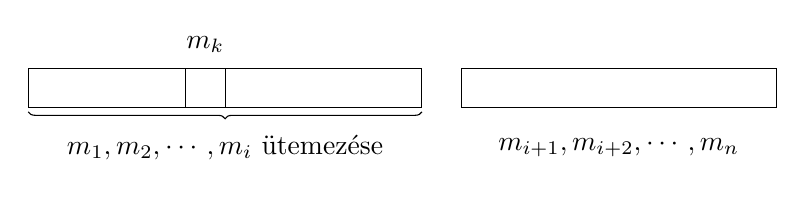
\begin{tikzpicture}
\draw (0,0) rectangle ++(5,0.5);
\draw (5.5,0) rectangle ++(4,0.5);

\draw[decoration={brace, raise=0.05cm, mirror}, decorate] (0, 0) -- (5, 0);
\node at (2.5, -0.5) {$m_1, m_2, \cdots, m_i$ ütemezése};
\node at (7.5, -0.5) {$m_{i+1}, m_{i+2}, \cdots, m_n$};

\draw (2.0, 0) -- (2.0, 0.5);
\draw (2.5, 0) -- (2.5, 0.5);
\node at (2.25, 0.8) {$m_k$};
\end{tikzpicture}
}

$\mathcal{O}^*$:
\raisebox{-.85\height}{
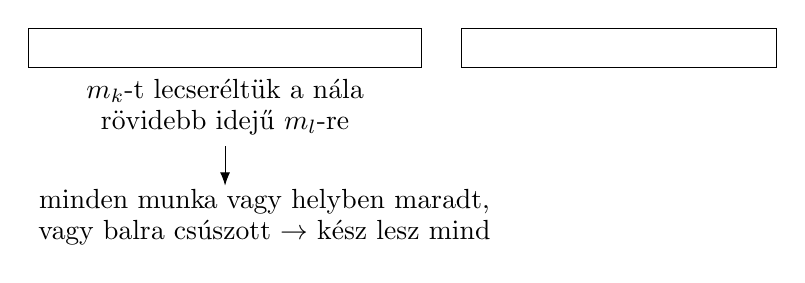
\begin{tikzpicture}
\draw (0,0) rectangle ++(5,0.5);
\draw (5.5,0) rectangle ++(4,0.5);
\node at (2.5, -0.3) {$m_k$-t lecseréltük a nála};
\node at (2.5, -0.7) {rövidebb idejű $m_l$-re};
\node at (3.0, -1.7) {minden munka vagy helyben maradt,};
\node at (3.0, -2.1) {vagy balra csúszott $\rightarrow$ kész lesz mind};

\draw[-Latex] (2.5, -1.0) -- (2.5, -1.5);

\end{tikzpicture}
}

$\mathcal{O}^*$ is optimális, és $\mathcal{O}^*$ nem tartalmazza az $m_k$ munkát. QED


\end{document}